% Lines starting with a percent sign (%) are comments. LaTeX will 
% not process those lines. Similarly, everything after a percent 
% sign in a line is considered a comment. To produce a percent sign
% in the output, write \% (backslash followed by the percent sign). 
% ==================================================================
% Usage instructions:
% ------------------------------------------------------------------
% The file is heavily commented so that you know what the various
% commands do. Feel free to remove any comments you don't need from
% your own copy. When redistributing the example thesis file, please
% retain all the comments for the benefit of other thesis writers! 
% ==================================================================
% Compilation instructions: 
% ------------------------------------------------------------------
% Use pdflatex to compile! Input images are expected as PDF files.
% Example compilation:
% ------------------------------------------------------------------
% > pdflatex thesis-example.tex
% > bibtex thesis-example
% > pdflatex thesis-example.tex
% > pdflatex thesis-example.tex
% ------------------------------------------------------------------
% You need to run pdflatex multiple times so that all the cross-references
% are fixed. pdflatex will tell you if you need to re-run it (a warning
% will be issued)  
% ------------------------------------------------------------------
% Compilation has been tested to work in ukk.cs.hut.fi and kosh.hut.fi
% - if you have problems of missing .sty -files, then the local LaTeX
% environment does not have all the required packages installed.
% For example, when compiling in vipunen.hut.fi, you get an error that
% tikz.sty is missing - in this case you must either compile somewhere
% else, or you cannot use TikZ graphics in your thesis and must therefore
% remove or comment out the tikz package and all the tikz definitions. 
% ------------------------------------------------------------------

% General information
% ==================================================================
% Package documentation:
% 
% The comments often refer to package documentation. (Almost) all LaTeX
% packages have documentation accompanying them, so you can read the
% package documentation for further information. When a package 'xxx' is
% installed to your local LaTeX environment (the document compiles
% when you have \usepackage{xxx} and LaTeX does not complain), you can 
% find the documentation somewhere in the local LaTeX texmf directory
% hierarchy. In ukk.cs.hut.fi, this is /usr/texlive/2008/texmf-dist,
% and the documentation for the titlesec package (for example) can be 
% found at /usr/texlive/2008/texmf-dist/doc/latex/titlesec/titlesec.pdf.
% Most often the documentation is located as a PDF file in 
% /usr/texlive/2008/texmf-dist/doc/latex/xxx, where xxx is the package name; 
% however, documentation for TikZ is in
% /usr/texlive/2008/texmf-dist/doc/latex/generic/pgf/pgfmanual.pdf
% (this is because TikZ is a front-end for PGF, which is meant to be a 
% generic portable graphics format for LaTeX).
% You can try to look for the package manual using the ``find'' shell
% command in Linux machines; the find databases are up-to-date at least
% in ukk.cs.hut.fi. Just type ``find xxx'', where xxx is the package
% name, and you should find a documentation file.
% Note that in some packages, the documentation is in the DVI file
% format. In this case, you can copy the DVI file to your home directory,
% and convert it to PDF with the dvipdfm command (or you can read the
% DVI file directly with a DVI viewer).
% 
% If you can't find the documentation for a package, just try Googling
% for ``latex packagename''; most often you can get a direct link to the
% package manual in PDF format.
% ------------------------------------------------------------------


% Document class for the thesis is report
% ------------------------------------------------------------------
% You can change this but do so at your own risk - it may break other things.
% Note that the option pdftext is used for pdflatex; there is no
% pdflatex option. 
% ------------------------------------------------------------------
\documentclass[12pt,a4paper,oneside,pdftex]{report}

% The input files (tex files) are encoded with the latin-1 encoding 
% (ISO-8859-1 works). Change the latin1-option if you use UTF8 
% (at some point LaTeX did not work with UTF8, but I'm not sure
% what the current situation is) 
\usepackage[utf8]{inputenc}
% OT1 font encoding seems to work better than T1. Check the rendered
% PDF file to see if the fonts are encoded properly as vectors (instead
% of rendered bitmaps). You can do this by zooming very close to any letter 
% - if the letter is shown pixelated, you should change this setting 
% (try commenting out the entire line, for example).  
\usepackage[T1]{fontenc}
% The babel package provides hyphenating instructions for LaTeX. Give
% the languages you wish to use in your thesis as options to the babel
% package (as shown below). You can remove any language you are not
% going to use.
% Examples of valid language codes: english (or USenglish), british, 
% finnish, swedish; and so on.
\usepackage[finnish,swedish,english]{babel}

% enable more precise float placements with "H" placement option
 \usepackage{float}


% Font selection
% ------------------------------------------------------------------
% The default LaTeX font is a very good font for rendering your 
% thesis. It is a very professional font, which will always be 
% accepted. 
% If you, however, wish to spicen up your thesis, you can try out
% these font variants by uncommenting one of the following lines
% (or by finding another font package). The fonts shown here are 
% all fonts that you could use in your thesis (not too silly). 
% Changing the font causes the layouts to shift a bit; you many
% need to manually adjust some layouts. Check the warning messages
% LaTeX gives you.
% ------------------------------------------------------------------
% To find another font, check out the font catalogue from
% http://www.tug.dk/FontCatalogue/mathfonts.html
% This link points to the list of fonts that support maths, but
% that's a fairly important point for master's theses.
% ------------------------------------------------------------------
% <rant>
% Remember, there is no excuse to use Comic Sans, ever, in any
% situation! (Well, maybe in speech bubbles in comics, but there 
% are better options for those too)
% </rant>

% \usepackage{palatino}
% \usepackage{tgpagella}



% Optional packages
% ------------------------------------------------------------------
% Select those packages that you need for your thesis. You may delete
% or comment the rest.

% Natbib allows you to select the format of the bibliography references.
% The first example uses numbered citations: 
% \usepackage[square,sort&compress,numbers]{natbib}
% The second example uses author-year citations.
% If you use author-year citations, change the bibliography style (below); 
% acm style does not work with author-year citations.
% Also, you should use \citet (cite in text) when you wish to refer
% to the author directly (\citet{blaablaa} said blaa blaa), and 
% \citep when you wish to refer similarly than with numbered citations
% (It has been said that blaa blaa~\citep{blaablaa}).
% \usepackage[square]{natbib}
\usepackage[round,authoryear]{natbib}

% The alltt package provides an all-teletype environment that acts
% like verbatim but you can use LaTeX commands in it. Uncomment if 
% you want to use this environment. 
% \usepackage{alltt}

% The eurosym package provides a euro symbol. Use with \euro{}
\usepackage{eurosym} 

% Verbatim provides a standard teletype environment that renderes
% the text exactly as written in the tex file. Useful for code
% snippets (although you can also use the listings package to get
% automatic code formatting). 
\usepackage{verbatim}

% The listing package provides automatic code formatting utilities
% so that you can copy-paste code examples and have them rendered
% nicely. See the package documentation for details.
\usepackage{listings}

\lstset{
  captionpos=b,
  aboveskip=1em,
  belowskip=1em
  }

% listings caption formatting
\usepackage{caption}
\captionsetup[lstlisting]{position=bottom}

% Support JSON examples
\usepackage{xcolor}

\colorlet{punct}{red!60!black}
\definecolor{background}{HTML}{EEEEEE}
\definecolor{delim}{RGB}{20,105,176}
\colorlet{numb}{magenta!60!black}

\lstdefinelanguage{json}{
    basicstyle=\normalfont\ttfamily,
    numbers=left,
    numberstyle=\scriptsize,
    stepnumber=1,
    numbersep=8pt,
    showstringspaces=false,
    breaklines=true,
    frame=lines,
    backgroundcolor=\color{background},
    literate=
     *{0}{{{\color{numb}0}}}{1}
      {1}{{{\color{numb}1}}}{1}
      {2}{{{\color{numb}2}}}{1}
      {3}{{{\color{numb}3}}}{1}
      {4}{{{\color{numb}4}}}{1}
      {5}{{{\color{numb}5}}}{1}
      {6}{{{\color{numb}6}}}{1}
      {7}{{{\color{numb}7}}}{1}
      {8}{{{\color{numb}8}}}{1}
      {9}{{{\color{numb}9}}}{1}
      {:}{{{\color{punct}{:}}}}{1}
      {,}{{{\color{punct}{,}}}}{1}
      {\{}{{{\color{delim}{\{}}}}{1}
      {\}}{{{\color{delim}{\}}}}}{1}
      {[}{{{\color{delim}{[}}}}{1}
      {]}{{{\color{delim}{]}}}}{1},
}

\definecolor{lightgray}{rgb}{.9,.9,.9}
\definecolor{darkgray}{rgb}{.4,.4,.4}
\definecolor{purple}{rgb}{0.65, 0.12, 0.82}

\lstdefinelanguage{JavaScript}{
  keywords={typeof, new, true, false, catch, function, return, null, catch, switch, var, if, in, while, do, else, case, break},
  keywordstyle=\color{blue}\bfseries,
  ndkeywords={class, export, boolean, throw, implements, import, this},
  ndkeywordstyle=\color{darkgray}\bfseries,
  identifierstyle=\color{black},
  sensitive=false,
  comment=[l]{//},
  morecomment=[s]{/*}{*/},
  commentstyle=\color{purple}\ttfamily,
  stringstyle=\color{red}\ttfamily,
  morestring=[b]',
  morestring=[b]"
}

% use smaller line spacing in lists
\let\oldenumerate\enumerate
\renewcommand{\enumerate}{
  \oldenumerate
  \setlength{\itemsep}{1pt}
  \setlength{\parskip}{0pt}
  \setlength{\parsep}{0pt}
}

\let\olditemize\itemize
\renewcommand{\itemize}{
  \olditemize
  \setlength{\itemsep}{1pt}
  \setlength{\parskip}{0pt}
  \setlength{\parsep}{0pt}
}


% The fancuvrb package provides fancier verbatim environments 
% (you can, for example, put borders around the verbatim text area
% and so on). See package for details.
% \usepackage{fancyvrb}

% Supertabular provides a tabular environment that can span multiple 
% pages. 
%\usepackage{supertabular}
% Longtable provides a tabular environment that can span multiple 
% pages. This is used in the example acronyms file. 
\usepackage{longtable}

% The fancyhdr package allows you to set your the page headers 
% manually, and allows you to add separator lines and so on. 
% Check the package documentation. 
% \usepackage{fancyhdr}

% Subfigure package allows you to use subfigures (i.e. many subfigures
% within one figure environment). These can have different labels and
% they are numbered automatically. Check the package documentation. 
\usepackage{subfigure}

% The titlesec package can be used to alter the look of the titles 
% of sections, chapters, and so on. This example uses the ``medium'' 
% package option which sets the titles to a medium size, making them
% a bit smaller than what is the default. You can fine-tune the 
% title fonts and sizes by using the package options. See the package
% documentation.
\usepackage[medium]{titlesec}

% The TikZ package allows you to create professional technical figures.
% The learning curve is quite steep, but it is definitely worth it if 
% you wish to have really good-looking technical figures. 
\usepackage{tikz}
% You also need to specify which TikZ libraries you use
\usetikzlibrary{positioning}
\usetikzlibrary{calc}
\usetikzlibrary{arrows}
\usetikzlibrary{decorations.pathmorphing,decorations.markings}
\usetikzlibrary{shapes}
\usetikzlibrary{patterns}


% The aalto-thesis package provides typesetting instructions for the
% standard master's thesis parts (abstracts, front page, and so on)
% Load this package second-to-last, just before the hyperref package.
% Options that you can use: 
%   mydraft - renders the thesis in draft mode. 
%             Do not use for the final version. 
%   doublenumbering - [optional] number the first pages of the thesis
%                     with roman numerals (i, ii, iii, ...); and start
%                     arabic numbering (1, 2, 3, ...) only on the 
%                     first page of the first chapter
%   twoinstructors  - changes the title of instructors to plural form
%   twosupervisors  - changes the title of supervisors to plural form
%\usepackage[mydraft]{aalto-thesis}
\usepackage[mydraft,doublenumbering]{aalto-thesis}
%\usepackage{aalto-thesis}


% Hyperref
% ------------------------------------------------------------------
% Hyperref creates links from URLs, for references, and creates a
% TOC in the PDF file.
% This package must be the last one you include, because it has
% compatibility issues with many other packages and it fixes
% those issues when it is loaded.   
\RequirePackage[pdftex]{hyperref}
% Setup hyperref so that links are clickable but do not look 
% different
\hypersetup{colorlinks=false,raiselinks=false,breaklinks=true}
\hypersetup{pdfborder={0 0 0}}
\hypersetup{bookmarksnumbered=true}
% The following line suggests the PDF reader that it should show the 
% first level of bookmarks opened in the hierarchical bookmark view. 
\hypersetup{bookmarksopen=true,bookmarksopenlevel=1}
% Hyperref can also set up the PDF metadata fields. These are
% set a bit later on, after the thesis setup.   


% Thesis setup
% ==================================================================
% Change these to fit your own thesis.
% \COMMAND always refers to the English version;
% \FCOMMAND refers to the Finnish version; and
% \SCOMMAND refers to the Swedish version.
% You may comment/remove those language variants that you do not use
% (but then you must not include the abstracts for that language)
% ------------------------------------------------------------------
% If you do not find the command for a text that is shown in the cover page or
% in the abstract texts, check the aalto-thesis.sty file and locate the text
% from there. 
% All the texts are configured in language-specific blocks (lots of commands
% that look like this: \renewcommand{\ATCITY}{Espoo}.
% You can just fix the texts there. Just remember to check all the language
% variants you use (they are all there in the same place). 
% ------------------------------------------------------------------
\newcommand{\TITLE}{Raising the Abstraction Level for Visualizing Geographical Data on the Web}
\newcommand{\FTITLE}{Abstraktiotason nostaminen geografisen datan web-visualisoinnissa}
\newcommand{\SUBTITLE}{Reducing the work needed by eliminating boilerplate}
\newcommand{\FSUBTITLE}{Tarvittavan boilerplate-koodin vähentäminen}
\newcommand{\DATE}{October 14, 2014}
\newcommand{\FDATE}{14. lokakuuta 2014}

% Supervisors and instructors
% ------------------------------------------------------------------
% If you have two supervisors, write both names here, separate them with a 
% double-backslash (see below for an example)
% Also remember to add the package option ``twosupervisors'' or
% ``twoinstructors'' to the aalto-thesis package so that the titles are in
% plural.
% Example of one supervisor:
%\newcommand{\SUPERVISOR}{Professor Antti Ylä-Jääski}
%\newcommand{\FSUPERVISOR}{Professori Antti Ylä-Jääski}
%\newcommand{\SSUPERVISOR}{Professor Antti Ylä-Jääski}
% Example of twosupervisors:
\newcommand{\SUPERVISOR}{Professor Petri Vuorimaa}
\newcommand{\FSUPERVISOR}{Professori Petri Vuorimaa}

% If you have only one instructor, just write one name here
\newcommand{\INSTRUCTOR}{Sami Vihavainen D.Sc. (Tech.)}
\newcommand{\FINSTRUCTOR}{Tekniikan tohtori Sami Vihavainen}
% If you have two instructors, separate them with \\ to create linefeeds
% \newcommand{\INSTRUCTOR}{Olli Ohjaaja M.Sc. (Tech.)\\
%  Elli Opas M.Sc. (Tech)}
%\newcommand{\FINSTRUCTOR}{Diplomi-insinööri Olli Ohjaaja\\
%  Diplomi-insinööri Elli Opas}
%\newcommand{\SINSTRUCTOR}{Diplomingenjör Olli Ohjaaja\\
%  Diplomingenjör Elli Opas}

% If you have two supervisors, it is common to write the schools
% of the supervisors in the cover page. If the following command is defined,
% then the supervisor names shown here are printed in the cover page. Otherwise,
% the supervisor names defined above are used.
% \newcommand{\COVERSUPERVISOR}{Professor Antti Ylä-Jääski, Aalto University\\
%  Professor Pekka Perustieteilijä, University of Helsinki}

% The same option is for the instructors, if you have multiple instructors.
% \newcommand{\COVERINSTRUCTOR}{Olli Ohjaaja M.Sc. (Tech.), Aalto University\\
%  Elli Opas M.Sc. (Tech), Aalto SCI}


% Other stuff
% ------------------------------------------------------------------
\newcommand{\PROFESSORSHIP}{Media}
\newcommand{\FPROFESSORSHIP}{Media}
% Professorship code is the same in all languages
\newcommand{\PROFCODE}{T-111}
\newcommand{\KEYWORDS}{work, in, progress}
\newcommand{\FKEYWORDS}{vähän, vielä, kesken}
\newcommand{\LANGUAGE}{English}
\newcommand{\FLANGUAGE}{Englanti}
\newcommand{\SLANGUAGE}{Engelska}

% Author is the same for all languages
\newcommand{\AUTHOR}{Pyry Kröger}


% Currently the English versions are used for the PDF file metadata
% Set the PDF title
\hypersetup{pdftitle={\TITLE\ - \SUBTITLE}}
% Set the PDF author
\hypersetup{pdfauthor={\AUTHOR}}
% Set the PDF keywords
\hypersetup{pdfkeywords={\KEYWORDS}}
% Set the PDF subject
\hypersetup{pdfsubject={Master's Thesis}}


% Layout settings
% ------------------------------------------------------------------

% When you write in English, you should use the standard LaTeX 
% paragraph formatting: paragraphs are indented, and there is no 
% space between paragraphs.
% When writing in Finnish, we often use no indentation in the
% beginning of the paragraph, and there is some space between the 
% paragraphs. 

% If you write your thesis Finnish, uncomment these lines; if 
% you write in English, leave these lines commented! 
% \setlength{\parindent}{0pt}
% \setlength{\parskip}{1ex}

% Use this to control how much space there is between each line of text.
% 1 is normal (no extra space), 1.3 is about one-half more space, and
% 1.6 is about double line spacing.  
% \linespread{1} % This is the default
% \linespread{1.3}
\linespread{1.2}

% Bibliography style
% acm style gives you a basic reference style. It works only with numbered
% references.
% \bibliographystyle{acm}
% Plainnat is a plain style that works with both numbered and name citations.
\bibliographystyle{plainnat}


% Extra hyphenation settings
% ------------------------------------------------------------------
% You can list here all the files that are not hyphenated correctly.
% You can provide many \hyphenation commands and/or separate each word
% with a space inside a single command. Put hyphens in the places where
% a word can be hyphenated.
% Note that (by default) LaTeX will not hyphenate words that already
% have a hyphen in them (for example, if you write ``structure-modification 
% operation'', the word structure-modification will never be hyphenated).
% You need a special package to hyphenate those words.
\hyphenation{di-gi-taa-li-sta yksi-suun-tai-sta}



% The preamble ends here, and the document begins. 
% Place all formatting commands and such before this line.
% ------------------------------------------------------------------
\begin{document}
% This command adds a PDF bookmark to the cover page. You may leave
% it out if you don't like it...
\pdfbookmark[0]{Cover page}{bookmark.0.cover}
% This command is defined in aalto-thesis.sty. It controls the page 
% numbering based on whether the doublenumbering option is specified
\startcoverpage

% Cover page
% ------------------------------------------------------------------
% Options: finnish, english, and swedish
% These control in which language the cover-page information is shown
\coverpage{english}


% Abstracts
% ------------------------------------------------------------------
% Include an abstract in the language that the thesis is written in,
% and if your native language is Finnish or Swedish, one in that language.

% Abstract in English
% ------------------------------------------------------------------
\thesisabstract{english}{
A dissertation or thesis is a document submitted in support of candidature
for a degree or professional qualification presenting the author's research and
findings. In some countries/universities, the word thesis or a cognate is used
as part of a bachelor's or master's course, while dissertation is normally
applied to a doctorate, whilst, in others, the reverse is true.

\fixme{Abstract text goes here (and this is an example how to use fixme).} 
Fixme is a command that helps you identify parts of your thesis that still
require some work. When compiled in the custom \texttt{mydraft} mode, text
parts tagged with fixmes are shown in bold and with fixme tags around them. When
compiled in normal mode, the fixme-tagged text is shown normally (without
special formatting). The draft mode also causes the ``Draft'' text to appear on
the front page, alongside with the document compilation date. The custom
\texttt{mydraft} mode is selected by the \texttt{mydraft} option given for the
package \texttt{aalto-thesis}, near the top of the \texttt{thesis-example.tex}
file.

The thesis example file (\texttt{thesis-example.tex}), all the chapter content
files (\texttt{1introduction.tex} and so on), and the Aalto style file
(\texttt{aalto-thesis.sty}) are commented with explanations on how the Aalto
thesis works. The files also contain some examples on how to customize various
details of the thesis layout, and of course the example text works as an
example in itself. Please read the comments and the example text; that should
get you well on your way!}

% Abstract in Finnish
% ------------------------------------------------------------------
\thesisabstract{finnish}{Tämä on diplomityö.}

% Acknowledgements
% ------------------------------------------------------------------
% Select the language you use in your acknowledgements
\selectlanguage{english}

% Uncomment this line if you wish acknoledgements to appear in the 
% table of contents
%\addcontentsline{toc}{chapter}{Acknowledgements}

% The star means that the chapter isn't numbered and does not 
% show up in the TOC
\chapter*{Acknowledgements}

So long, and thanks for all the fish.

\vskip 10mm

\noindent Espoo, \DATE
\vskip 5mm
\noindent\AUTHOR

% Acronyms
% ------------------------------------------------------------------
% Use \cleardoublepage so that IF two-sided printing is used 
% (which is not often for masters theses), then the pages will still
% start correctly on the right-hand side.
\cleardoublepage
% Example acronyms are placed in a separate file, acronyms.tex
\addcontentsline{toc}{chapter}{Abbreviations and Acronyms}
\chapter*{Abbreviations and Acronyms}

% The longtable environment should break the table properly to multiple pages, 
% if needed

\noindent
\begin{longtable}{@{}p{0.25\textwidth}p{0.7\textwidth}@{}}
2k/4k/8k mode & COFDM operation modes \\
3GPP & 3rd Generation Partnership Project \\ 
ESP & Encapsulating Security Payload; An IPsec security protocol \\ 
FLUTE  & The File Delivery over Unidirectional Transport protocol \\ 
e.g.& for example (do not list here this kind of common acronymbs or abbreviations, but only those that are essential for understanding the content of your thesis. \\ 
note & Note also, that this list is not compulsory, and should be omitted if you have only few abbreviations

\end{longtable}


% Table of contents
% ------------------------------------------------------------------
\cleardoublepage
% This command adds a PDF bookmark that links to the contents.
% You can use \addcontentsline{} as well, but that also adds contents
% entry to the table of contents, which is kind of redundant.
% The text ``Contents'' is shown in the PDF bookmark. 
\pdfbookmark[0]{Contents}{bookmark.0.contents}
\tableofcontents

% List of tables
% ------------------------------------------------------------------
% You only need a list of tables for your thesis if you have very 
% many tables. If you do, uncomment the following two lines.
% \cleardoublepage
% \listoftables

% Table of figures
% ------------------------------------------------------------------
% You only need a list of figures for your thesis if you have very 
% many figures. If you do, uncomment the following two lines.
% \cleardoublepage
% \listoffigures

% The following label is used for counting the prelude pages
\label{pages-prelude}
\cleardoublepage

%%%%%%%%%%%%%%%%% The main content starts here %%%%%%%%%%%%%%%%%%%%%
% ------------------------------------------------------------------
% This command is defined in aalto-thesis.sty. It controls the page 
% numbering based on whether the doublenumbering option is specified
\startfirstchapter

% Add headings to pages (the chapter title is shown)
\pagestyle{headings}

% The contents of the thesis are separated to their own files.
% Edit the content in these files, rename them as necessary.
% ------------------------------------------------------------------
%!TEX root = thesis.tex

\chapter{Introduction}
\label{chapter:intro}

% The introduction in itself is rarely very long; two to five pages often
% suffice.

We are confronted with a quickly increasing amount of data every day. We also increasingly need to use the data as a basis for our actions and thoughts. Data visualization enables us to obtain insight about data quickly and efficiently \citep{van_wijk_value_2005}, making it crucial in the modern world. 

An estimated 95 \% of all digital data contains geographical references \citep{perkins_have_2010}. Visualizing this data helps users perceive geospatial relationships and patterns. Additionally, geographical visualizations can be used for determining information on distances, directions and areas \citep[chap.~1.1]{kraak_cartography_2011}. Using geographical visualizations, it is also possible to organize data spatially and visually, allowing more efficient memorization of data.

Geographical data is data with geospatial dimension, such as Point of Interest (POI) with location data as coordinates \citep[chap.~1.2]{kraak_cartography_2011}. The most natural method for visualizing geographical data is usually with various maps. In the past, geographical data was predominantly visualized by cartographers, but it has been recognized \citep{kraak_visualization_1999} that the situation has changed, with people from increasing number of fields having a need -- and the possibility \citep[chap.~1]{slocum_thematic_2014} -- for visualizing geographical data. Moreover, the popularity of Google Maps \citep{google_maps_2005-1} along with its Application Programming Interface (API) \citep{google_maps_2005} has proved that in addition to experts of other academic fields, there is a definite demand for web map visualizations within consumers as well. 

The web makes publishing and bundling map visualizations extraordinarily straightforward when compared to traditional desktop-based Geographic Information System (GIS) applications: traditional desktop-based GIS system requires an installation of the GIS application and often additional tools and accounts for publishing the visualization, while using web-based mapping software ideally requires no additional software or tools or even accounts. This is especially important when the visualizations are made by non-cartographers who only make visualizations occasionally and lack the needed resources and experience for more complex publishing process \citep{miller_beast_2006}. However, as the web platform is primarily designed for static documents \citep{berners-lee_information_1989,berners-lee_world-wide_1992} instead of dynamic applications \citep{jazayeri_trends_2007}, there are some additional concerns to address when making a complex data visualization on the web.

\section{Problem Statement}

Currently, there are several libraries available for displaying maps and simple visualizations \citep{google_maps_2005,agafonkin_leaflet_2011,metacarta_openlayers_2006}. However, the problem is that none of the mainstream libraries is of sufficiently high abstraction level for building map visualizations efficiently, resulting in the need for writing \emph{boilerplate} code that does not directly contribute to the visualization. Moreover, the libraries are not designed primarily for visualizations and therefore do not encourage or push the visualizer to create visually and cognitively effective visualizations, resulting in subpar visualizations \citep[chap.~1]{slocum_thematic_2014}.

\section{Objectives and Scope}

Our primary objective is to make creating map visualizations for the web more efficient by building a reusable higher abstraction level software system for map visualizations, and to evaluate the efficiency benefits of the system. This system should provide the structure for creating the visualization as well as common web application features needed in modern web applications. Our secondary objective is to encourage more effective visualizations by considering the cognitive requirements of visualizations when building the system.

In order to find the solution for the problem, it is necessary to study geographical visualizations and software reuse. The process of making geographical visualizations should be studied to ensure that the system encourages creating \emph{effective} visualizations. In addition, software reuse should be studied in order to be able to create versatile visualizations \emph{efficiently}. Therefore, to evaluate the objectives, we select the following research questions for this thesis:

\begin{enumerate}
	\item[RQ1] How does a reusable software system affect the \emph{efficiency} of building geographical visualizations?
	\item[RQ2] How does a reusable software system affect the \emph{effectiveness} of geographical visualizations?
\end{enumerate}

In the scope of this thesis, we adopt the process definitions of \citet{van_wijk_value_2005} by making the difference between an efficient and an effective process. \emph{By an efficient process, we mean a process which requires as little as possible effort and other resources to complete. By an effective process, we mean a process which reaches its objectives sufficiently.} Therefore, building a visualization efficiently indicates that the building process is as effortless as possible, and building an effective visualization indicates that the resulting visualization conveys its intended message appropriately.

% a) how does a reusable software system affect the efficiency of ...
% b) can a reusable software system...


\section{Approach}

In order to build an efficient system for visualizing geographical data, it is needed to study (a) how to visualize geographical data and (b) how to build reusable software. We begin by first studying the basics of data visualization with an emphasis on geographical data, maps and the visualization process. After visualization, we study the essence of software reuse, focusing on building and evaluating reusable software. Based on suggestions from earlier research, we proceed to create a reusable visualization tool and evaluate its effect on visualization effectiveness and efficiency of the building process.

\section{Structure of the Thesis}
\label{section:structure} 

Chapter \ref{chapter:intro} (this introduction) presents the motivation for this thesis as well as the problem statement. Chapter \ref{chapter:reuse} presents the essence of software reuse, concentrating on success factors and methods for reuse. Chapter \ref{chapter:dataviz} describes the fundamentals of data visualizations with an emphasis on geographic data and thematic mapping. In chapter \ref{chapter:reuseinvisualization}, we discuss the research on data visualization reuse along with its shortcomings, and argue about the need for this research.

In chapter \ref{chapter:methods}, we present some of the most prominent methods for evaluating software reuse and visualization effectiveness, selecting the most suitable methods for this work. In chapter \ref{chapter:implementation}, we describe the implementation of the tool designed to address the shortcomings presented in chapter \ref{chapter:reuseinvisualization}. In chapter \ref{chapter:evaluation}, we evaluate the implementation based on the methods presented in chapter \ref{chapter:methods} and analyze the evaluation results. In chapter \ref{chapter:discussion}, we interpret the evaluation results along with their applicability, shortcomings and generalizability. We also propose topics for further research based on this work. In chapter \ref{chapter:conclusions}, we conclude the findings and other implications of the thesis.

%!TEX root = thesis.tex

\chapter{Background}
\label{chapter:background} 

% Also known as ``literature review''/``Kirjallisuuskatsaus''. About 20 pages long.

In order to build an efficient framework for visualizing geographical data, it is needed to study (a) how to visualize geodata and (b) how to build frameworks. We are going to tackle this problem by first studying the basics of data visualization with an emphasis on geographical data, maps and the visualization process. After visualization, we are going to study the essence of software reuse, focusing on building and evaluating reusable software, also known as software frameworks.

\section{Data Visualization}

\subsection{Definition}

According to \citet[chap.~3]{kosara_visualization_2007}, there is no universally accepted definition of visualization. He proposes the following for a ``minimal set of requirements for any visualization'':

\begin{itemize}
	\item It is based on (non-visual) data
	\item It produces an image
	\item The results are readable and recognizable
\end{itemize}

According to him, while visualizations can also have other properties or qualities, such as interaction or visual efficiency, the requirements above are the ones needed for technical definition of the term. Moreover, it should be emphasized that according to this definition, visualization is the \emph{process} itself, not the result of it.

\citet[chap.~4]{kosara_visualization_2007} argues that visualization is separated into two types, \emph{pragmatic} and \emph{artistic} visualization. Pragmatic visualization focuses on the analysis of the data in order to show its relevant characteristics as efficiently as possible. Artistic visualization on the other hand concentrates on the communication of the concern behind the data, not the display of the actual data. \citeauthor{kosara_visualization_2007} states that while these types focus on the opposite sides of the visualization spectrum, it may be possible to close the gap using e.g. interaction.

The first requirement for visualizations by \citet{kosara_visualization_2007} dictates that the visualization is based on data. This is an essential characteristic of \emph{data} visualizations: the visualization is a function which takes data as an input and produces a visual object as an output. In less technical terms, this means that the visualization turns data into visual, effortlessly and efficiently digestible format.

This leads to the fact that the data and visualization are not inherently tied to each other; the visualization ``function'' can be independent of the data and thus it may be possible to create a visualization framework or platform which is able to function on a potentially wide range of data.

\fixme{The goal of visualization is (usually) better understanding of the data.}

% This may need to moved to Thematic Map Visualization part:
% ``As this thesis concentrates on the display of data, the analysis of data is considered mainly outside the scope.''

\subsection{Principles for Successful Data Visualization}

The requirements presented in the previous section are sufficient for the definition of data visualization. However, they do not convey any information about visualization quality. In order to discover the characteristics for successful data visualization, additional principles are needed. \citet[p.~13]{tufte_visual_1986} states that excellent graphics (i.e. results of visualizations) consist of ``complex ideas communicated with clarity, precision and efficiency''. In practice, this means that the graphics should emphasize the actual data and its nuances above everything else, while serving a clear purpose.

In addition to graphics principles presented in the previous paragraph, \citet[p.~93]{tufte_visual_1986} presents the concept of \emph{data-ink}. Data-ink represents the ink used for displaying the data in a visualization. He argues that in an excellent visualization, most, if not all, ink used should contribute to display of the data. However, research by \citet{inbar_minimalism_2007} suggests that maximizing the share of data-ink may not be beneficial to the user experience of the visualization. 

The principles presented above are essential, but too abstract in order to be used as a sole basis for defining a good visualization. However, when combined with the data visualization definition stated above, the principles become considerably more useful and concrete. \citet{azzam_j-b_2013} propose an adapted version of the definition by \citet{kosara_visualization_2007}, complementing the second requirement by requiring the produced image to represent the data truthfully. This definition effectively combines the definition by \citet{kosara_visualization_2007} with the principle of showing data introduced by \citet{tufte_visual_1986}. The adapted definition facilitates the process of creating a successful data visualizations by offering a more concrete version of Tufte's principles. It gives the developer of the visualization a concrete checklist for representing the data: make sure it does not (a) omit or (b) overrepresent any information \citep{azzam_j-b_2013}.

% \fixme{This section could really use some more content}

\fixme{If desperately in need of more background, add human perception in relation to information visualization (from Ware).}

\subsection{Visualizing Geographical Data}

\fixme{Visualization - Scientific Visualization - Map Visualization - \citet{kraak_cartographic_1998} has a good overview.}

The most natural way of visualizing geographical data is by using a map\citep[chap.~1]{kraak_cartographic_1998,kraak_cartography_2011}. This technique is called \emph{thematic mapping} \citep[chap.~1]{slocum_thematic_2014}. Thematic mapping does not require any specific format of data, except for the geographical dimension \citep[chap.~1]{kraak_cartography_2011}. However, the nature of the data has a great effect on the method, or type, of thematic mapping.

\subsubsection{Methods for Thematic Mapping}

As stated above, there are several types of geographical data, many of which are fundamentally different requiring different visualization methods. Therefore, several different thematic mapping methods have been developed. \citet[chap.~14-18]{slocum_thematic_2014} list some of the most typical ones: \fixme{rephrase the descriptions below}

\begin{itemize}
	\item Choropleth map - Shows data aggregated for a set of predefined areas (countries, regions etc)
	\item Isarithmic map - Maps with areas separated by contour lines.
	\item Dasymetric map - \fixme{what's this?}
	\item Proportional symbol map - like dot map, but replaces dots with relevant symbols of sizes proportional to the data
	\item Dot map - simple maps with dots on relevant locations
	\item Multivariate mapping - A map that shows data of several dimensions (in addition to location).
	\item Flow map - a map that shows ``flows'' from one area to another. Napoleon Russian campaign map.
\end{itemize}

When designing a software framework for geovisualization, it is not necessary to support every method above. However, as those are some of the most used ones, omitting any must be a conscious decision.

\fixme{describe the use cases for each type}

Even a single thematic map is often used for multiple different purposes \citep[chap.~2]{schlichtmann_visualization_2002}. For instance, a single map can be read on the \emph{overall level} (``where are the primary schools located in Helsinki metropolitan area?'') and \emph{elementary level} (``is there a primary school in Punavuori?''). Furthermore, some possible uses for a thematic map are ``what is the ratio and distribution of Finnish schools compared to Swedish schools in Helsinki'' or ``what is the spatial distribution of sizes of schools in Helsinki''. Therefore, an efficient map visualization should not lock the user to any single perspective. \fixme{maybe move somewhere? Create a separate (sub)section for interactivity?} \fixme{Interactivity could help here? See \citep{andrienko_interactive_1999}}

\fixme{Analysis part of geovisualization - ``...is considered out of the scope of this work.''}

~

\fixme{To Do}
\begin{itemize}
	\item Geographic visualization (e.g. in relation to scientific visualization)
	\item Map visualization vs. map (thematic map vs general-reference map) \citep{bartz_petchenik_place_1979}
	\item How do the principles introduced in the previous subsection apply to geographical data? Is there anything else to consider?
	\item Thematic map interactivity \citep{andrienko_interactive_1999} (Where should this go? Is this an env related thing or here somewhere)
\end{itemize}

\citet[p.~16]{tufte_visual_1986} May help here as well.

\section{How Thematic Maps Are Made}
\citet{schlichtmann_visualization_2002} describes making thematic maps as a six-step process. The first four steps involve deciding on and obtaining the data which are not relevant when building a software framework for visualization. Therefore, we ignore those steps. The step five consists of selecting the visualization method and using it to produce a meaningful visualization from the data. The step six involves explaining the visualization in legend. \fixme{Schlichtmann not concerned with the step 6, find some other source of displaying the legend.}

In the map visualization process, several identified objectives for the resulting graphic exist \citep{schlichtmann_visualization_2002}. The objectives are presented in the table below.

\LTcapwidth=\textwidth
\begin{longtable}{|p{3cm}|p{10cm}|}
\hline
\textbf{Name} & \textbf{Description} \\ 
\hline
Clarification & Making the map clear and readable. In practice, this means that the topemes (symbols) in a map should be easily detectable and distinguishable from each other \\
\hline
Emphasis & Making topemes and other important characteristics of the visualization to stand out visually \\
\hline
Types of Entries & Having a clearly distinguishable type for each topeme. \\
\hline
Sets of Types & Grouping data points and symbols with similar traits in order to make them belong together visually. Ideally, the visual similarity should be related to the conceptual similarity. \\
\hline
Cross-Relations & Visually indicating the potential relations and similarities between different types or between entries of different types. \\
\hline
Local Syntax & Aligning visual properties of the topemes to prevent unintentional emphasis of single topemes. \\
\hline
Local Ensembles & Supporting topemes with multiple properties (such as the numbers of children and adults in an area) so that the topeme visually reflect both the individual properties and the combination of all properties. \\
\hline
Multilocal Ensembles & Supporting topemes with multiple geographical properties (such as spatial distribution of people)  \\
\hline
Addable and Non-Addable Quantities & Differentiating addable and non-addable properties. Typically absolute quantitative properties are addable while relative and qualitative properties are non-addable. Addable properties should be visualized in a way that cognitively supports addition (e.g. with sizes of elements) while non-addable quantities should be visualized without said feature (e.g. with colors.) \\
\hline
The Surface Illusion & Creating an illusion of surface on the map. This can be achieved for example by using illumination and shadowing. These visual traits can convey a meaning themselves and often naturally do so. \\
\hline
\caption{Map visualization objectives as per \citet{schlichtmann_visualization_2002}}
\end{longtable}

The objectives above are important when visualizing geographical data on a map. Therefore, it is needed to take those into account when creating a visualization tool or framework in order to enable or even encourage the visualizers to reach as many of the objectives as possible.

\fixme{This could use an opinion from some other source as well (Maybe \citep[p.~5]{slocum_thematic_2014})}

\section{Software Reuse}

In order to create a reusable software framework for visualization, it is necessary to study software reuse along with different reuse techniques and their characteristics, advantages and disadvantages.

\citet{krueger_software_1992} presents software reuse as a process of reusing existing software code (applications, libraries, functions or single lines) when building new software, while according to \citet{mohagheghi_empirical_2008}, reuse is not restricted to code, but can also refer to other software assets such as design. However, both agree that software reuse combines several different existing pieces of code (and possibly other assets) along with new assets which are specific for the application in question. According to \citet{mcilroy_mass-produced_1969} and \citet{boehm_managing_1999}, it is one of the most effective techniques of reducing the development time and cost of complex software products.

\subsection{Software Reuse Advantages \& Disadvantages}

When used appropriately, software reuse has several benefits. In their overview of multiple case studies, \citet{mohagheghi_empirical_2008} discovered that in most cases, using reused software components resulted in a considerably lower number of software defects and better productivity. Several of the studies implied that reusing software is also beneficial for software complexity and product time-to-market. However, it should be noted that since the overview only addresses case studies, its results should not be considered universally applicable.

Although reusing software is often said to decrease the effort needed \citep{mcilroy_mass-produced_1969, boehm_managing_1999, mohagheghi_empirical_2008} \fixme{there must be many more sources for this available}, concrete evidence for this is difficult to find \citep{mohagheghi_empirical_2008}.

Given its lucrative advantages, software reuse is definitely beneficial for many software systems. However, according to \citet{krueger_software_1992}, software reuse can be problematic and even disadvantageous. Learning to use a specific piece of reusable software often takes considerable effort. Moreover, finding suitable code fragments may also prove to be a challenge. For uncomplicated software systems and especially reusable components, it may not be worth the effort. Therefore, developer needs to carefully consider all sides of reusing when building a software system; according to \citet[chap.~1.3]{krueger_software_1992}, for successful software reuse scenario, the amount of intellectual effort between the concept and implementation of the system must be as low as possible. In practice, this means that the value of the reused component must be as high as possible for the developed system, while the implementation cost (resources needed to take the reusable component into use) should be relatively low. 

\subsection{Factors for Successful Software Reuse}
\citet{frakes_success_1994} state that for successful software reuse, the procedure must be planned beforehand and evaluated with a cost-benefit analysis. \fixme{They also present several other factors, add them here.} \fixme{This needs a lot more flesh. Add some general principles etc. ``How to make reusable software''}

\subsection{Analyzing Software Reuse}
According to \citet{krueger_software_1992}, in order to analyze reusing software, the reuse process to be studied should be separated into four \emph{dimensions}. The dimensions are presented below.

~

\textbf{Abstraction} is the process of making a piece of software more generic, thus making it applicable to a wider range of software projects. Software reuse is almost always based on abstraction, but according to \citet{krueger_software_1992}, raising the abstraction level has proven to be difficult, thus making building reusable software a nontrivial process.\newline

\textbf{Selection} facilitates finding, comparing and choosing suitable pieces of software. For example, libraries or frameworks aid selection by bundling and structuring the software components.\newline

\textbf{Specialization} is the process of making the abstracted component more specific, usually by parameterizing the software or making it transformable.\newline

\textbf{Integration} facilitates providing the software with reusable components, for example with a mechanism to import relevant modules or functions to the software.\newline

\fixme{Add advantages and disadvantages in general about reuse, not about different methods as those are described in the reuse methods chapter. Software reuse metrics research \citep{mohagheghi_empirical_2008,frakes_software_1996,selby_enabling_2005} probably has some good points. Also, \citet{johnson_frameworkscomponents+_1997} may have something.}

\subsection{Software Reuse Methods}

%Here should be analysis about libraries, components, frameworks... Use \citet{krueger_software_1992}. Also why choose framework? \citet{johnson_frameworkscomponents+_1997} has some reasons.

%\citet{krueger_software_1992} has a list of different methods along with their advantages and disadvantages. Includes frameworks in chapter 10. \citet{johnson_frameworkscomponents+_1997} extends the description. Using the characteristics along with praise of \citet{johnson_frameworkscomponents+_1997}, it should be possible to reason about going with frameworks.

~

Software reuse is not a single, uniform procedure or technique. Several different reuse techniques exist to cater different needs. Consequently, different reuse methods excel at different areas. In order to describe the advantages and disadvantages of the methods, we describe the using the reuse dimensions presented in the previous section.

\citet{krueger_software_1992} and \citet{johnson_frameworkscomponents+_1997}, among others, present and analyze software reuse methods. From these, we have selected the most relevant for web environment, presenting those below.

% High-level languages, design and code scavenging, source code components, software schemas, application generators, very high-level languages, transformational systems, software architectures

\subsubsection{High-Level Languages}
High-level languages denote programming languages which are designed to be on a high abstraction level and thus contain features which are not necessary for a programming language but benefit or speed up the development. Traditional examples of these kind of features are automatic memory allocation \citep{krueger_software_1992} and language constructs such as exceptions \citep{mitchell_concepts_2003}. More modern high-level language features are value type checking systems and abstracted support for parallel operations using futures \citep{totoo_haskell_2012}. It should be noted that the high-levelness of a language is a \emph{relative} property, i.e. it is not possible to determine the requirements for a high-level language per se, only high-levelness of languages compared to other languages. For example, \citet{krueger_software_1992} considers all programming languages above the abstraction level of the assembly language high-level languages, while \citet{carro_high-level_2006} consider e.g. lack of automatic memory management or type system a sign of lower-level language.

High-level languages \emph{abstract} frequently used procedures into seemingly uncomplicated operations, thus reducing the work and cognitive capacity needed for developing the application. \citep[chap.~3]{krueger_software_1992}

As the number of elementary high-level language constructs is usually relatively low it is possible for programmers to master the use of those constructs with sufficiently little effort, rendering \emph{selection} unproblematic. \citep[chap.~3]{krueger_software_1992}

\emph{Specialization} of high-level language features is usually achieved by parameterizing the constructs, either implicitly or explicitly. For example, when instantiating a class in Java, the only parameterization needed for memory management is the actual object instance. However, e.g. exception handling always requires at least the logic needed for handling the exception. \citep[chap.~3]{krueger_software_1992}

\emph{Integration} of high-level language features is automatically done when compiling the software code. However, due to the nature of high-level languages, it is usually not possible to mix-and-match different programming languages easily in the same program. \citep[chap.~3]{krueger_software_1992}

The advantages of high-level languages are mainly related to the decreased need for developing frequently needed procedures manually, such as allocating or deallocating memory, case-by-case. These operations in high-level languages can be mapped into more complex procedures in some lower-level languages, effectively making them reusable software components. In practice, using high-level languages can yield a productivity gain up to 500 \%. \citep[chap.~3]{krueger_software_1992}

The main disadvantage of using high-level languages is the potential decrease in performance. As with any software reuse, high-level programming languages abstract the supported procedures by making them more generic. This often leads to additional complexity and unnecessary operations on the compiled program. However, the decrease can often be minimized by using additional compile-time optimizations. \citep{carro_high-level_2006}

On the web, the technologies used on the client-side are inherently fixed to descendants of HTML, CSS and JavaScript \citep{world_wide_web_consortium_html5_2014,world_wide_web_consortium_cascading_2011,ecma_ecmascript_2011}. Therefore, web application languages are relatively high-level by definition. However, it is still possible to raise the abstraction level by using e.g. CoffeeScript \citep{ashkenas_coffeescript_2009} instead of JavaScript or LESS \citep{sellier_less_2009} instead of CSS.

\subsubsection{Design and Code Scavenging}

Design and Code scavenging refers to the technique of scavenging pieces of software \emph{ad hoc} from existing software systems and using the pieces as parts for a new software system  \citep[chap.~4]{krueger_software_1992}. The aim of this technique is to reduce the amount of work needed to build the system. For example, when building an UI component for choosing a date, the developer may scavenge the code for a calendar from an older software system.

Scavenging can be done without modifications to the code in the target code base (code scavenging) or by modifying the details of the scavenged code (design scavenging) \citep[chap.~4]{krueger_software_1992}. The \emph{abstraction} gained by scavenging is therefore mostly informal and in some cases even its existence is questionable \citep[chap.~3]{sametinger_software_1997}. Usually, there is no ``hidden part'' of the abstraction but the developer must maintain the functionality of all the code himself \citep[chap.~3]{sametinger_software_1997}.

Usually there is no formal mechanism or support for \emph{selecting} pieces of software to be scavenged. Therefore, the developer must rely on his memory, experience and word-of-mouth in order to find suitable pieces of software. \citep[chap.~3]{sametinger_software_1997}

\emph{Specialization} is done by manually editing the scavenged source code. While it is often the fastest method of acquiring results, this requires the developer to deeply understand the scavenged implementation. It can also lead to fragmentation and maintainability issues in the future. \citep[chap.~4]{krueger_software_1992}

\emph{Integration} of the scavenged code is done by copying and pasting the code to the target source code file. This may lead to namespace collisions between original and scavenged code which may result in the need for refactoring the code. \citep[chap.~4]{krueger_software_1992}

The main advantages of design and code scavenging are the ability to quickly include existing functionality to new software systems \citep[chap.~4]{krueger_software_1992}. As it is usually not needed to prepare the code to be scavenged before scavenging it, the extent of possible pieces of software is often significantly larger than when using any other reuse method. 

However, finding suitable pieces of software for scavenging is hard. Moreover, scavenging pieces of software often does not decrease the \emph{cognitive distance} between the target and implementation of the system. It may also create issues with maintainability of the software. \citep[chap.~4]{krueger_software_1992}

\subsubsection{Source Code Components}

Using source code components is a type of reuse that chooses and uses software components from a component repository \citep[chap.~3]{sametinger_software_1997}. Software component can be any piece of code, but in practice, components usually consist of one or more functions, modules or classes \citep[chap.~3]{sametinger_software_1997}. An example of a source code component is a trigonometry module which contains functions for sine, cosine and tangent calculations. When a developer needs to calculate sines in her program, she searches a component repository for trigonometry components and utilizes the component found in her own program \citep[chap.~5]{krueger_software_1992}.

Ideally, source code components \emph{abstract} the implementation details of the component inside. This means that the required cognitive distance between the concept and the implementation of the software system is lower when using source code components instead of e.g. code scavenging. 

In order to be \emph{selectable}, source code components should be accompanied by abstract names (function names) and descriptions of the functionality provided \citep[chap.~5]{krueger_software_1992}. The names should describe \emph{what} the components does instead of \emph{how} it does it \citep[chap.~5]{krueger_software_1992}. These names can then be used for reasoning about the purpose of the component and finding the component in source code component repositories -- in order to use the component, the developer must be able to find it and to know what it does \citep[chap.~5]{krueger_software_1992}.

Source code components can be \emph{specialized} by modifying the source code \citet[chap.~5]{krueger_software_1992}. However, as this technique yields unwanted consequences explained in the previous section, many components support specialization by parameterization. For example, the programmer could provide the sine function the angle in question. Additionally, when integrating the trigonometry module to her software system, the programmer could specify if the functions should use degrees or radians. In some components, specialization can also be achieved via subclassing \citep[chap.~5]{krueger_software_1992}.

All modern programming languages support \emph{integration} of reusable source code components written in the same language. Usually, the procedure is a very simple addition of source code files, which requires little to no effort on the programmer side. However, all source code components can't be used in the same program due to conflicts e.g. in naming and value types \citep[chap.~5]{krueger_software_1992}.

The main advantages of using source code components are the abstraction provided and organized nature of the component repositories. Ideally, the repositories provide a search functionality so that even developers with no previous experience on the component domain can find the components needed. Moreover, the abstraction level and the hiding of implementation details decreases the cognitive distance between the concept and the implementation of the system and reduce the source code needed to be written.

The main disadvantages of the source code components lie in the fact that the functionality must be deliberately designed to support reuse. The abstraction of the components is a major challenge \citep[chap.~5]{krueger_software_1992} in designing source code components. Additionally, the component repositories need administration and maintenance.

\subsubsection{Software Schemas}

\fixme{Add similarly structured content as in the previous subsubsection. Or maybe drop?}

\subsubsection{Application Generators}

Application generators are usually domain-specific generators which take very high level instructions (specifications) as input and then output significantly lower level software code (implementation) \citep[chap.~7]{cleaveland_building_1988,krueger_software_1992}. On fundamental level, application generators differ from high-level language compilers mainly by being designed to work on a narrow domain and thus being able to support considerably higher-level instructions \citep[chap.~7]{krueger_software_1992}. Unlike source code components, the reused components generated by application generators are usually not encapsulated or separated \citep[chap.~3]{sametinger_software_1997}.

Application generators \emph{abstract} the concept or specification of the software system, hiding the actual implementation completely from the user of the generator \citep{cleaveland_building_1988}. However, in some cases it may be necessary to modify the output of the generator which essentially removes the abstraction.

In principle, \emph{selecting} application generations is moderately easy since the abstraction level of application generators is usually very high, rendering reasoning about the purpose of the generator fairly easy \citep[chap.~7]{krueger_software_1992}. However, since application generators are usually suited for a very narrow domain, it is usually difficult to find a suitable generator \citep[chap.~7]{krueger_software_1992}.

Typically, software systems generated with application generators consist of variant and invariant parts \citep[chap.~7]{krueger_software_1992}. Invariant part is the part of the program which the developer using the generator can't modify. The developer \emph{specializes} the program by modifying the variant part. There are several methods of modifying the variant part. One of the simplest may be straightforward parameterization: the developer chooses the parameters of the system from a predefined set of alternatives. This method makes using the generation extraordinarily easy. However, it also limits the resulting application considerably.

On the other end of the spectrum, the application generator may require the variant parts to be inputted using a domain-specific or generic-purpose programming language. This makes the application generator incredibly versatile, but requires both more domain-specific and programming knowledge.

Typically, application generators generate complete applications which do not require further \emph{integration} \citep[chap.~7]{krueger_software_1992}. However, occasionally, the resulting applications are not independent per se, but require integration to other systems. This may be an issue since often it is not possible to select the integration interfaces freely, but to use the ones provided by the generator.

One of the main advantages of the application generators is the abstraction they provide. In some cases, the application generators may even require no programming language knowledge as long as the user has relevant domain-specific knowledge \citep{horowitz_survey_1985}. Moreover, application generators excel when there is a need for building multiple similar applications \citep[chap.~7]{krueger_software_1992}. 

However, application generators require the an unambiguous mapping between the specifications and implementation details \citep[chap.~7]{krueger_software_1992}. Moreover, building application generators requires a reliable, generic implementation and user interfaces for developers \citep{cleaveland_building_1988}. Therefore, building application generators requires comprehensive domain-specific knowledge in addition to extensive software development expertise.

\subsubsection{Very High Level Languages}

\fixme{Or domain-specific languages? Add similarly structured content as in the previous subsubsection}

\subsubsection{Transformational Systems}

\fixme{Add similarly structured content as in the previous subsubsection. Or maybe drop?}

\subsubsection{Software Architectures}

\fixme{Add similarly structured content as in the previous subsubsection}

\subsubsection{Software Frameworks}

\fixme{Add similarly structured content as in the previous subsubsection. Are frameworks the same as architectures? If, drop.}

%\subsection{Software Frameworks}

%Frameworks more in depth. Maybe how to build them.

%\fixme{Is it OK to describe frameworks in depth, but not other means of reuse? How to reason about this? Could it be done so that frameworks do not have a separate chapter (here), but instead go through all methods. Then, in the implementation chapter, reason about which methods to use (most likely more than just framework here)}

\section{Evaluating Software Reuse Effectiveness}

Here should be the whole research on how to measure if it is beneficial to reuse software instead of writing from scratch. At least \citet{mohagheghi_empirical_2008,frakes_software_1996,selby_enabling_2005} are useful here.


%!TEX root = thesis.tex

%\chapter{Web Applications}
%\label{chapter:environment}

%Describe HTML5, JS and other related technology, because these are really the things that restrict the implementation.

% This could be entirely about web tech for maps? About 5 pages long.

%\fixme{Maybe drop this chapter, or merge a short version of it to implementation}

%Visualizations need to be implemented using web technology, because it is crucial for distributability and discoverability that the system works in web browsers... \fixme{continue...}

%\section{Geographic Visualization on the Web}

%Probably should describe the relevant web technology, some needed HTML5/JS features etc. \fixme{to subsection of related webtech?}

%!TEX root = thesis.tex

\chapter{Methods}
\label{chapter:methods}

In this chapter, I describe the methodological approach used for finding the answers to my research questions. I also argue about the reasons for selecting the methods, and reasons for excluding the other methods presented in section \ref{section:evaluatingreuse}. 

\emph{From a broad methodological perspective, this study follows the constructive approach. This means that a system is implemented and evaluated \citep{jarvinen_tutkimustyon_2012}. In more detail, I evaluated the implementation system through six case studies. In the evaluation stage, I employed both quantitative and qualitative data gathering and analysis methods.} The evaluation of process efficiency (RQ1) is measured quantitatively, examining the numeric characteristics of several case studies. The visualization effectiveness (RQ2) is evaluated qualitatively, analyzing whether the tool encourages the visualizer to conform to visualization guidelines.

Next, I will describe the methodological setting in more detail.

\section{Constructive Study}

\emph{In order to find answers to the research questions\footnote{How does a reusable software system affect the \emph{efficiency} of building geographical visualizations?}\footnote{How does a reusable software system affect the \emph{effectiveness} of geographical visualizations?}, I decided to conduct a constructive study by implementing and evaluating a reusable geovisualization tool.} Constructive research excels at finding answers to questions of type ``how useful is system X'' \citep{jarvinen_tutkimustyon_2012}, making it the most suitable research type for this thesis.

In practice, conducting a constructive study involves designing an artifact and evaluating its effect \citep{jarvinen_tutkimustyon_2012}. \emph{In this study, I built a reusable geographical visualization tool}, evaluating its effect on the effectiveness of the visualization and the efficiency of building the visualization. This can be done by performing a \emph{case study}, i.e., observing one or more visualization cases and evaluating the relevant properties in those cases. In this study, I selected six visualization cases to evaluate the effect of the implemented tool on effectiveness and efficiency of visualization. The cases were: 1) store map depicting the locations of Alko stores, 2) map of earthquakes in California after January 1, 1900, 3) regional voter turnout in the Finnish presidential election of 2012, 4) regional share of people with no secondary education in Finland, 5) travel times to a single destination in Helsinki metropolitan area, and 6) average travel times to multiple destinations in Helsinki metropolitan area. To enable as realistic evaluation as possible, all cases presented use real-life data in formats obtainable from the Web.

\section{Evaluating Software Reuse Effectiveness}

In section \ref{section:successfullreusefactors}, I concluded that it is critical to analyze and measure software reuse. In this study, I utilized both high-level and low-level analysis methods. High-level methods emphasize the development process and higher-level properties of software, while low-level methods are more concerned with the methods for measuring individual software projects. In addition, I select the metrics for measuring software code properties needed by the higher-level methods.

\subsection{High-level Evaluation}
As presented in section \ref{section:evaluatingreuse}, several methods for high-level software reuse analysis exist. \emph{In this study, I used the cost-benefit analysis method}. Cost-benefit analysis models consider both development costs for the reusable component and the reuse productivity and quality benefits. Unlike the other methods presented, such as the maturity assessment model, it is suitable for assessing a single piece of software instead of a complete software reuse program or a reusable software library.

\subsection{Low-level Evaluation}

The models presented above are high-level analysis tools which do not take a stance on how to measure the detailed data required by the measurements. Hence, the models need to be complemented with lower-level, more detail-oriented methods. \emph{Of the methods presented by \citet{mohagheghi_quality_2007}, I decided to use the case study method.} As the scope of this work does not allow for large sample sizes required by controlled experiment method, it is not a feasible alternative for this study. Moreover, using experience reports requires a considerable experience on creating and using reusable software which is not possible to achieve for this work.

\emph{I conducted the case studies through the sister project comparison method}, as according to \citet{mohagheghi_quality_2007}, it is suitable for evaluating a specific piece of reusable software. For the evaluation, I built several visualizations with and without the reusable tool, evaluating the difference in approaches.

\subsection{Software Code Metrics}

As described in section \ref{section:evaluatingreuse}, software code properties can be measured with several different metrics. In order to achieve as reliable evaluation as possible, I decided to use a diverse set of different software code metrics. As suggested by \citet{fenton_software_1998}, I evaluated the implementations by measuring the number of both physical and effective lines of code.

According to \citet{fenton_software_1998}, software code line counts should be complemented with metrics related to functionality and complexity of the software. \emph{Therefore, I decided to use the cyclomatic complexity measure of \citet{mccabe_complexity_1976} for determining the application complexity.} The method is superior to other methods presented mainly because it provides a computable measure with which it is possible to measure implementation details of a program. As discussed in chapter \ref{section:evaluatingreuse}, the ``problem complexity'' approach of \citet{fenton_software_1998} is not appropriate for evaluating different implementations of the same problem and thus it was not selected.

\emph{In addition to the metrics presented above, I decided to employ the \citeauthor{halstead_elements_1977} metrics for difficulty and effort.} The main advantage of these methods when compared to the previous methods is that they provide an explicit, direct measure for the properties. Like the metric of \citeauthor{mccabe_complexity_1976}, \citeauthor{halstead_elements_1977} metrics are computable from the program source code, making them effective for this study.

The COCOMO approaches of \citet{boehm_software_1981} were not used because they are either too vague (Basic COCOMO 81) or too process-centric (Intermediate and Detailed COCOMO 81, COCOMO II) for this study.

\section{Evaluating the Effectiveness of a Visualization}

I decided to examine whether the reusable visualization tool is advantageous to the effeciveness of the visualization, i.e., if visualizations built with the tool are likely to be more effective in conveying the information than visualizations built without the tool. To some degree, this can be done with several different methods. \emph{In this study, I decided to use visualization heuristics by \citet{zuk_heuristics_2006} and thematic mapping objectives by \citet{schlichtmann_visualization_2002} due to the fact that those are the most concrete guidelines presented.}

In addition to the methods selected, several other methods exist. While some of the methods are more concrete than others, it is notable that none of the methods provides formal, computable means for evaluation. According to \citet{kraak_cartographic_1998}, \emph{evaluating geographical visualizations is predominantly done by estimating the visualization subjectively in relation to its context}. This makes objective effectiveness evaluation complicated.

The principles by \citet{tufte_visual_1986}, such as data-ink ratio presented in section \ref{section:visualizationprinciples} can be used to evaluate the visualization. Another method for evaluation is presented by \citet{azzam_j-b_2013}. However, the correctness of these methods is disputed \citep{kosslyn_graphics_1985,inbar_minimalism_2007}. Moreover, the methods are too abstract for effective formal evaluation.

Visualization heuristics by \citet{zuk_heuristics_2006} presented in section \ref{section:visualizationprinciples} are significantly more concrete than the methods presented in the previous paragraph and can be used for efficiently analyzing a visualization. \emph{Therefore, I decided to use the heuristics for evaluating the tool's effect on visualization effectiveness.}

Geovisualization-specific evaluation methods consist of the methods of \citet{kraak_cartographic_1998} and \citet{schlichtmann_visualization_2002}. While the former is useful for designing a visualization, it is too abstract for assessing visualizations effectively. The latter consists of a number of mapping objectives presented in section \ref{subsection:effectivemaps}. When compared to the former, it is considerably more concrete, enabling more effective formal evaluation. \emph{Therefore, I decided to complement the heuristics presented in the previous paragraph with the mapping objectives by \citet{schlichtmann_visualization_2002}}.

Due to the fact that the sister project method selected for efficiency evaluation aims to produce as similar results as possible, I deemed it unpractical to use the sister projects for evaluating the visualization effectiveness. \emph{Therefore, I decided to evaluate the tool qualitatively by examining whether it benefits the visualizer in terms of conforming to the heuristics and achieving the objectives.} This conforms to the statement of \citet{kraak_cartographic_1998} related to subjective evaluation of geovisualization.

 
%!TEX root = thesis.tex

\chapter{Implementation}
\label{chapter:implementation}

% 10-15 pages?

% You have now explained how you are going to tackle your problem. 
% Go do that now! Come back when the problem is solved!

% Now, how did you solve the problem? 
% Explain how you implemented your solution, be it a software component, a
% custom-made FPGA, a fried jelly bean, or whatever.
% Describe the problems you encountered with your implementation work.

As discussed in the chapter \ref{chapter:reuse}, reusing software typically leads to increased productivity and better quality. Therefore, to achieve the targets of this thesis, we decided to implement a reusable visualization tool. Our target was to create multiple different visualizations both with and without the tool in order to analyze its benefits.

\section{Problem Setting}

Currently, when building a visualization for geographical data, it is unnecessarily laborious to develop the visualization from the beginning using low abstraction level APIs provided by mapping libraries. This leads to the situation when using especially more complicated visualization methods such as isarithmic maps, it is not feasible to create an effective visualization, encouraging to use a simpler, yet more ineffective methods such as dot maps.

Second, when building web-based geographical visualizations, it is typically needed to build the whole visualization architecture using web technology such as HTML \citep{world_wide_web_consortium_html5_2014} and JavaScript \citep{ecma_ecmascript_2011}. Therefore, an astonishing amount of knowledge of such technology is required to even develop a simple map visualization. 

\fixme{Do these require some concrete or literature proof?}

\section{Application Requirements and Design}
\label{section:requirements}

We started the implementation process by analyzing the requirements of the different geographic visualization methods presented in chapter \ref{subsection:mappingmethods}. Specifically, we analyzed the underlying structure of the visualizations in order to abstract the applicable parts as reusable components. For this, we adopted the ``hot spot'' method by \citet{schmid_systematic_1997} for detecting similarities and dissimilarities in software.

In order to solve both problems presented in the previous section, we decided to implement a dual approach for visualization. First, as one of the problems related to visualizations is the amount of application architecture work needed, the tool should provide a so-called whole-page scaffold architecture \citep{jazayeri_trends_2007} which contains the needed page-specific architecture. We call this part of the system \emph{framework}. Second, we decided to implement an individual visualization component in order to support embedding the visualizations in existing web pages. We call this part \emph{library}. When referring to both of the parts of the system, we use the term \emph{application}.

\subsection{Reuse Methods}

We gathered the analyzed data about the requirements in addition to problems discussed in the previous chapter, and determined the forms of reuse applicable in this case. Since the techniques are not mutually exclusive and each has its own benefits, we decided to use a combination of multiple techniques. 

The application is developed, and can be used with, JavaScript language, which is relatively high-level programming language. The scaffold architecture uses the framework method for enabling the visualizer to get started with the visualization quickly while allowing thorough customization later if needed. The visualization library is built as a collection of software components, which allow versatile functionality and composability while abstracting the implementation details. Moreover, the tool contains example visualizations which can be used as a starting point for building visualizations.

\fixme{Maybe why drop other methods?}

\subsection{Supported visualization methods}
\label{subsection:supportedvisualizationmethods}

As discussed in the chapter \ref{subsection:mappingmethods}, several different thematic mapping methods exist. As some of these methods are fundamentally different in implementation, it is needed to explicitly consider the requirements of each method. It is also necessary to decide whether to implement support for each method, as it may be necessary to drop support for some of the methods in order to manage the application complexity and the scope of this work. We decided to implement support for the following visualization methods:

\begin{itemize}
	\item Choropleth maps
	\item Dasymetric maps
	\item Isarithmic maps
	\item Dot maps
	\item Proportional Symbol maps
\end{itemize}

\fixme{Should this include a little about why choosing these? Or is it enough to state the reasons in visualization chapter?}

Of the visualization methods presented in the chapter \ref{subsection:mappingmethods}, we decided to exclude explicit multivariate maps, cartograms and flow maps. The decision was made primarily due to the fact that of the methods presented in chapter \ref{subsection:mappingmethods}, these are the least frequently used. Moreover, since there are several fundamentally different design options for those methods, it is considerably more difficult to abstract the implementation details to provide a general-purpose visualization module. However, it should be noted that the modular architecture of the application enables easy extendability to support these type of visualizations in the future. Additionally, multivariate maps can be achieved to some degree by using several of the map methods simultaneously.

\section{Application Architecture}

In the highest level, the application architecture consists of two parts: the visualization framework and the visualization library. While the framework uses the library for visualization, it also consists of other functionality and the library can be used separately of the framework. The architecture of the framework is presented in figure \ref{fig:framework_architecture}.

Framework consists of a Web Single-Page Application (SPA) which embeds the visualization library along with other functionality necessary or beneficial for user experience. Notably, the application uses CSS for displaying the page correctly and HTML5 Application Cache\footnote{\url{http://diveintohtml5.info/offline.html}} for offline availability and faster loading times. \fixme{Any other?} Application also contains functionality for displaying the visualization correctly on devices of different sizes and capabilities.

\begin{figure}[htbp]
  \centering
  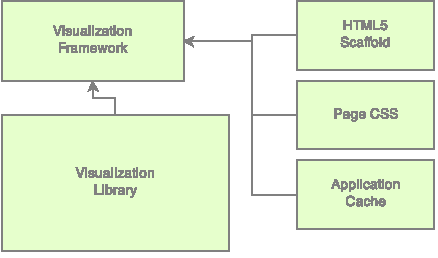
\includegraphics[width=\textwidth]{images/framework-architecture.pdf}
  \caption{The architecture of the visualization framework.}
  \label{fig:framework_architecture}
\end{figure}

\fixme{Add architecture diagram and description for the framework}

\begin{figure}[htbp]
  \centering
  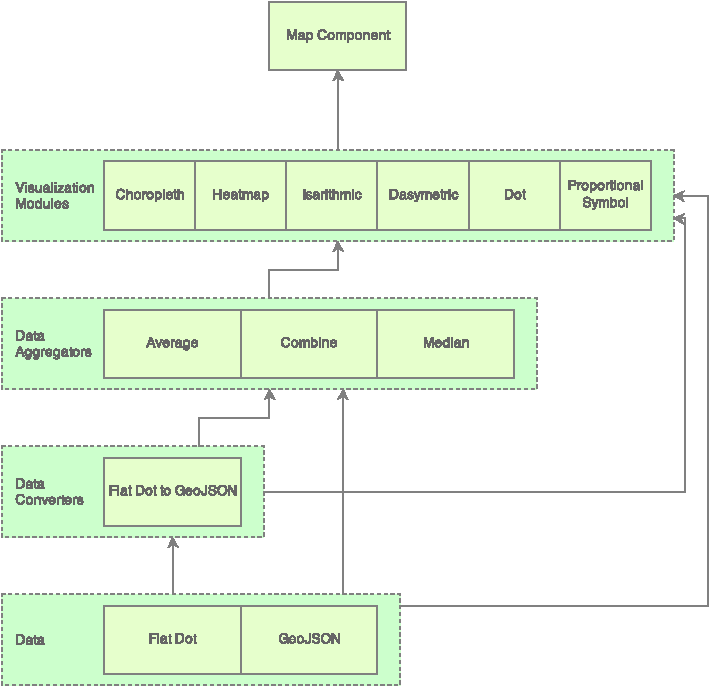
\includegraphics[width=\textwidth]{images/library-architecture.pdf}
  \caption{The architecture of the Thematic.js library. Arrows denote the flow of data.}
  \label{fig:lib_architecture}
\end{figure}

The architecture of the library is described in figure \ref{fig:lib_architecture}. The library consists of map component, mapping modules, data aggregators and data converters. The map component is used for displaying the map layer and for managing mapping modules and can be added to any block-level element on a web page. Internally, the map is displayed using Leaflet\footnote{\url{http://leafletjs.com/}}. 

Individual mapping modules are added to the map as Leaflet layers. For convenience and maintainability, we created an abstract mapping module for handling system-specific procedures such as keeping module status. The abstract module should be used as an object prototype for all mapping modules. Individual mapping modules each support a mapping method, but all can be customized to a degree. Currently, the modules only support GeoJSON\footnote{Geographic JavaScript Object Notation, \url{http://www.geojson.org}} data, but there are no technical restrictions on using any format of data.

Typically, mapping modules are used with some external data. The data is often in a non-standard format as presented in the chapter \ref{chapter:evaluation} \fixme{Ref to the chapter where test cases are presented}. For this, data converters are used. Data converters are straightforward stateless components which transform data from a non-standard format to format supported by the mapping modules. For example, the library provides a converter from ``flat dot'' JSON format \fixme{add appendix} to standard GeoJSON FeatureCollections.

Aggregators are similar to converters in the sense that both transform data. However, while converters do 1-to-1 conversions, aggregators combine several grouped data sets into one by, e.g., calculating an average of the values in sets.
	
The use of converters and aggregators is not required when creating a visualizations if the data is in the correct format, but the components help bring a structured way of transforming the data into appropriate format.

\section{Supported Platforms}

The application is developed using standard web technology. Theoretically, this means that the app supports all HTML5, CSS3 and ECMAScript6 compliant browsers. However, in practice, none of the widely used browsers support the standards completely \citep{manian_html5_2011}. Therefore, we have tested the application on the most widely used modern web browsers, i.e., the latest versions of Google Chrome (38), Mozilla Firefox (33), Safari (7.1), Opera (25), Internet Explorer (11), Mobile Safari (8) and Mobile Chrome (38). In total, this represents the browsers of NN \% of the Internet users \citep{statcounter_globalstats_2014}. \fixme{Check the browsers and versions actually supported and the resulting percentage}.

While the application is most naturally run in a web environment, it is also possible to embed the system to various native applications using a web view component. Web view components are available on at least Windows \citep{small_ten_2012}, Mac OS X \citep{hunter_why_2014}, Android \citep{google_building_2014} and Apple iOS \citep{apple_uiwebview_2014} platforms.

Due to the dual approach described in chapter \ref{section:requirements}, the application can be used in almost any existing web application, using almost any framework and library. However, due to possible namespace collision, other libraries using global namespaces \texttt{L} (Leaflet), \texttt{\char`_} (underscore), or \texttt{thematic} may cause an incompatibility with the application as described in \citet{osmani_essential_2011}.

\section{Implemented Functionality}

The following sections present the most important application functionality, namely supported mapping methods, managing input formats and values, and modularity for supporting future extensions.

\subsection{Choropleth Maps}

Choropleth maps are used for visualizing enumerated or areally aggregated data \citep[chap.~6]{dent_cartography:_2008}. According to \citet[chap.~14]{slocum_thematic_2014}, it is the most frequently used mapping method. Therefore, implementing choropleth mapping functionality is essential for a successful mapping tool.

To use choropleth mapping, visualizer uses the choropleth mapping module of the application. If the user already has the relevant data in GeoJSON format, nothing else is required. However, if the relevant data is stored separately of the designated area definitions, the user needs to use the \emph{combine} aggregator provided by the application. The aggregator associates the data with the area definition in question and outputs the data in GeoJSON format supported by the mapping module.

\fixme{add screenshot of a choropleth map}

\subsection{Dasymetric Maps}

Dasymetric maps are supported in an approximated fashion: the dasymetric mapping module \fixme{check name} approximates dasymetric data by using the floating grid method as presented by \citet{langford_generating_1994}. The module is provided the grid of dots in GeoJSON format as data, and the data is used to generate appropriate dasymetric map approximation. The data can also be aggregated and converted using any of the supplied aggregators and converters.

\fixme{add screenshot of a dasymetric map}

\subsection{Isarithmic Maps}

The application uses the Heatmap method for producing isarithmic maps. \fixme{Check Porkola's thesis for heat map literature etc. Can it be categorized as an isarithmic map? If no, move to a separate subsection. Then Isarithmic maps can be produced with isarithmic GeoJSON or approximating with Dasymetric maps}

\subsection{Dot Maps and Proportional Symbol Maps}

The application supports producing dot and proportional symbol maps by providing the Symbol mapping module. With default configuration, the module produces dot maps, but it is possible to provide an option for calculating and using proportional symbol values. For enabling the user getting more information about data points, it is possible enable information bubbles which are activated by click the symbol. The module also supports using customized symbols for data points, the default being a simple Leaflet marker.

\subsection{Input Formats}

All implemented mapping modules use GeoJSON as their input format. GeoJSON is the \emph{de facto} format for transmitting geographical data on the web \citep{bostock_code_2013}. There is also great support for GeoJSON data in the existing software, for example in Leaflet map library used by the application. However, due to its verboseness, GeoJSON may be unsuitable for simpler data sets and visualizations such as dot maps. Therefore, we have implemented a number of converters for transforming data to GeoJSON format. Currently, there is support for converting ``flat dot'' (see appendix \ref{appendix:flatdotformat}) and X formats \fixme{check which formats are supported.}

Typically, the data is fetched from an external resource (external API or a separate JSON file) asynchronously. Therefore, the modules support using ECMAScript Promises\footnote{\url{https://developer.mozilla.org/en/docs/Web/JavaScript/Reference/Global_Objects/Promise}} to pass visualized data. However, also synchronous data (such as using data defined in the source code file) is supported by wrapping the values in Promise objects.

\subsection{Value Normalization}

When visualizing a metric such as average temperature of an area, the scale of values is completely different from when visualizing, say, population density. Therefore, in order to provide general-purpose map visualization tools, it is necessary to support displaying a wide variety of values and scales.

For this application, we decided to implement a highly versatile normalization functionality which allows the visualizer to work on virtually any scale. Instead of transforming the input values into a predefined value set, the application transforms the input values directly to a visualizable value, such as ``red'' on a choropleth map, or ``10px'' on a proportional symbol map. Moreover, this mechanism is compatible with, e.g., scaling functionality of D3.js\footnote{\url{http://d3js.org/}, \url{https://github.com/mbostock/d3/wiki/Scales}} visualization library, so the visualizer can leverage the sophisticated scaling functionality of external libraries.

\subsection{Modularity and Extendability}

It is hardly possible to cover the whole area of geographic visualizations. Therefore, instead of trying to support every visualization method possible, we implemented the architecture of the application so that it is as straightforward as possible to extend the functionality.

As a result of this, visualization methods can be easily extended by adding tailored mapping modules to the application. Additionally, it is possible to create customized aggregators, converters and scales and bundle these as an extension to the application.

\section{Implementation Result}

Is this really usable? Has it been used? \fixme{Remove if no data}

~

\fixme{Would the implementation chapter need more practical examples, be it code or screenshots?}


%!TEX root = thesis.tex

\chapter{Evaluation}
\label{chapter:evaluation}

In this chapter, we describe the evaluation of the tool built. The evaluation is performed by using two separate methods: we evaluate the efficiency of development process with the software effort and complexity metrics presented in chapter \ref{chapter:methods}, and visualization effectiveness with heuristics by \citet{zuk_heuristics_2006} complemented by mapping objectives by \citet{schlichtmann_visualization_2002} presented in chapter \ref{section:visualizationprinciples}. As the first of the methods requires a baseline project, we decided to implement a number of sister projects as defined by \citet{kitchenham_evaluating_1998}. In this chapter, the visualizations built during sister projects are referred to with the term ``reference visualization'' while the visualizations built with Thematic.js are referred to with ``Thematic.js visualization''.

The most important findings of the evaluation are that 1) \emph{typically, Thematic.js improves the efficiency of building geographic visualizations significantly}, and 2) \emph{Thematic.js likely encourages creating effective visualizations}.

\section{Defining the Evaluated Cases}
\label{section:evaluatedcases}

The visualization tool should be able to visualize a large variety of data. Moreover, the benefits of reusable software are typically emphasized when examining a large number of relatively similar cases \citep{frakes_software_1996}. However, in order to keep the scope of this work manageable, we decided to evaluate a set of visualization cases listed below.

\paragraph{Alko stores in Finland}
Alko provides an unsupported representational state transfer (REST) API\footnote{\url{http://www.alko.fi/api/store/mapmarkers?language=fi}} for fetching data of Alko stores. The data is in a non-standard ``flat dot'' format (see appendix \ref{appendix:flatdotformat}). Therefore, we decided to visualize Alko store locations using a dot map. The map should display all Alko stores in an effective fashion, with clustering support for markers in order to avoid map cluttering. This case is later referred to as ``store map''.

\paragraph{Earthquakes in California}
Earthquakes have two fundamental data axes: location and magnitude. Therefore, earthquakes are best visualized using a proportional symbol map with the size of the symbol representing magnitude. United States Geological Survey provides historical earthquake data\footnote{\url{http://earthquake.usgs.gov/earthquakes/search/}}, and we decided to visualize earthquakes in the state of California since January 1, 1900. The data is available in a Comma-Separated Values (CSV) format which is can be trivially transformed to ``flat dot'' JSON format. This case is later referred to as ``earthquake map''.

\paragraph{Voter Turnout in Finnish Presidential Election of 2012}
The Finnish Ministry of Interior provides regional voter turnout data of the presidential election of 2012\footnote{\url{http://tulospalvelu.vaalit.fi/TP2012K2/s/aanaktiivisuus/aanestys1.htm}}. This data is provided in electoral district and municipality level. We decided to visualize the turnout in municipality level, using municipality data by the Finnish Land Survey\footnote{\url{http://www.maanmittauslaitos.fi/en/opendata}}. The municipality data is provided in GeoJSON format by Teemu Tiilikainen\footnote{\url{https://github.com/varmais/maakunnat}}. These data can be combined to create an effective choropleth visualization of regional turnout. The data should be normalized in quantized fashion, i.e., using thresholds to create a discrete color range. This case is later referred to as ``election map''.

\paragraph{Share of People with No Secondary Education in Finland}
Statistics Finland\footnote{\url{http://www.tilastokeskus.fi/}} provides provincial data on the education of the population of Finland in CSV format. This can be combined with province data by the Finnish Land Survey\footnote{\url{http://www.maanmittauslaitos.fi/en/opendata}} to create an effective choropleth visualization. The data should be normalized in linear fashion, i.e., using a continuous color range. This case is later referred to as ``education map''.

\paragraph{Travel Times to a Single Destination}
Travel times to a destination can be visualized using an isarithmic map. We decided to visualize travel times to Futurice headquarters\footnote{\url{http://futurice.com/contact\#helsinki}} using public transport. The travel times can be obtained by using Travel Time Visualization Utility for HSL Reittiopas\footnote{\url{https://github.com/pyryk/reittiopas-travel-times}} which provides the data in an approximated ``flat dot'' format. The data should be normalized in a quantized fashion to emphasize isarithmic contours. This case is later referred to as ``simple travel times map''.

\paragraph{Travel Times to Multiple Destinations}
In addition to visualizing travel times to a single destination, we decided to evaluate a case for displaying travel times to multiple destinations. The travel times are obtained with the method defined in the previous paragraph, and combined using a weighted average method. Like in the previous case, the data should be normalized in a quantized fashion. This case is later referred to as ``complex travel times map''.

~

While the visualized data is arbitrarily selected, the cases are picked to reflect the typical usage of visualizations. Choropleth map and isarithmic map are the most frequenly used thematic mapping methods \citep[chap.~14-15]{slocum_thematic_2014} and therefore it is beneficial to the evaluation to examine multiple visualizations with those methods.

In order to better model typical real-life use cases, and to be usable on the web, the visualization cases include also a generic application structure and HTML features such as application caching and bookmarking support which are highly beneficial features for web applications.

\section{Implementing Sister Projects}

We implemented six separate sister project visualizations with no visualization library to compare to visualization cases as defined in the previous section. The functionality of the visualizations was designed to reflect the functionality of the evaluated visualizations as accurately as possible. Sister visualizations were implemented using HTML, CSS and JavaScript to enable straightforward comparison to the evaluated visualization cases. While we did not use any visualization library for the sister projects, we deemed using a generic mapping library such as Leaflet.js appropriate, because typically, creating map visualizations is not feasible without using one. Moreover, also Thematic.js uses Leaflet.js as a mapping library.

In order to better reflect the actual situations involving building visualizations, the sister projects were implemented in \emph{ad hoc} fashion, meaning that the design or architecture of the applications were not planned extensively beforehand. Also, no reuse of any form between visualizations was planned. However, during implementation, some design and code scavenging was done in order to speed up the development process. The sister project code can be found in \url{https://github.com/pyryk/thesis-reference-implementations}.

\section{Evaluating Efficiency of Development}
\label{section:evaluatingefficiency}

We evaluated the efficiency of development by several metrics: software code length (number of physical (LOC) and logical (LLOC) lines of code), cyclomatic complexity (CC), Halstead difficulty (HD) and Halstead effort (HE). For measurements, we used ESComplex\footnote{\url{https://github.com/philbooth/escomplex}} for analyzing JavaScript programs. As the visualizations are implemented as single-page applications, the majority of the functionality lies within JavaScript, with only little HTML code and CSS definitions. Therefore, we decided to exclude HTML and CSS from the evaluation.

We began the evaluation by measuring the aforementioned metrics for the visualizations. It should be noted that for these measurements, we did not include code from Thematic.js or other third party libraries. The measurements are shown in table \ref{table:efficiencymetrics}.

\LTcapwidth=\textwidth
\begin{longtable}{|l|c|c|c|c|c|}
\hline
\textbf{Visualization} & \textbf{LOC} & \textbf{LLOC} & \textbf{CC} & \textbf{HD} & \textbf{HE} \\
\hline
\rowcolor{gray!15}
Thematic.js store & 12 & 12 & 1 & 7.31 & 4600 \\
\rowcolor{gray!15}
Reference store & 126 & 85 & 10 & 23.6 & 96500 \\
Thematic.js earthquake & 15 & 14 & 1 & 8.38 & 6280 \\
Reference earthquake & 79 & 121 & 10 & 23.5 & 87400 \\
\rowcolor{gray!15}
Thematic.js election & 26 & 29 & 2 & 10.9 & 12800 \\
\rowcolor{gray!15}
Reference election & 141 & 101 & 14 & 23.8 & 107000 \\
Thematic.js education & 17 & 17 & 1 & 10.2 & 10200 \\
Reference education & 129 & 87 & 10 & 27.8 & 109000 \\
\rowcolor{gray!15}
Thematic.js travel times simple & 27 & 28 & 2 & 10.8 & 9840 \\
\rowcolor{gray!15}
Reference travel times simple & 184 & 129 & 12 & 29.4 & 182000 \\
Thematic.js travel times complex & 30 & 30 & 2 & 11.6 & 13300 \\
Reference travel times complex & 193 & 144 & 12 & 34.5 & 255000 \\
\hline
\caption{Measurements for developed visualizations, including only visualization-specific code. The lower the value the better.}
\label{table:efficiencymetrics}
\end{longtable}

\emph{According to the results, using Thematic.js yields significantly lower complexity, difficulty and effort values when compared to using no visualization library.} This is likely a direct result of Thematic.js providing an extensive map-specific visualization functionality, allowing the visualizer to concentrate on the visualized data. In practice, this means that when creating map visualizations, it is significantly more efficient to use a library such as Thematic.js than to write the visualization from the ground up, given that the visualizer possesses -- or is able to achieve -- a general knowledge of the library functionality.

However, it is likely that the results do not describe the most typical real-life scenarios completely accurately. It can be assumed that typically, visualizers do not possess knowledge of Thematic.js functionality beforehand and therefore effort for each line of code is considerably higher than when building the visualization from the ground up. In the results, this is reflected in rather high values for relative difficulty for Thematic.js visualizations as seen in figure \ref{fig:evaluationchart}.

\begin{figure}[htbp]
  \begin{center}
    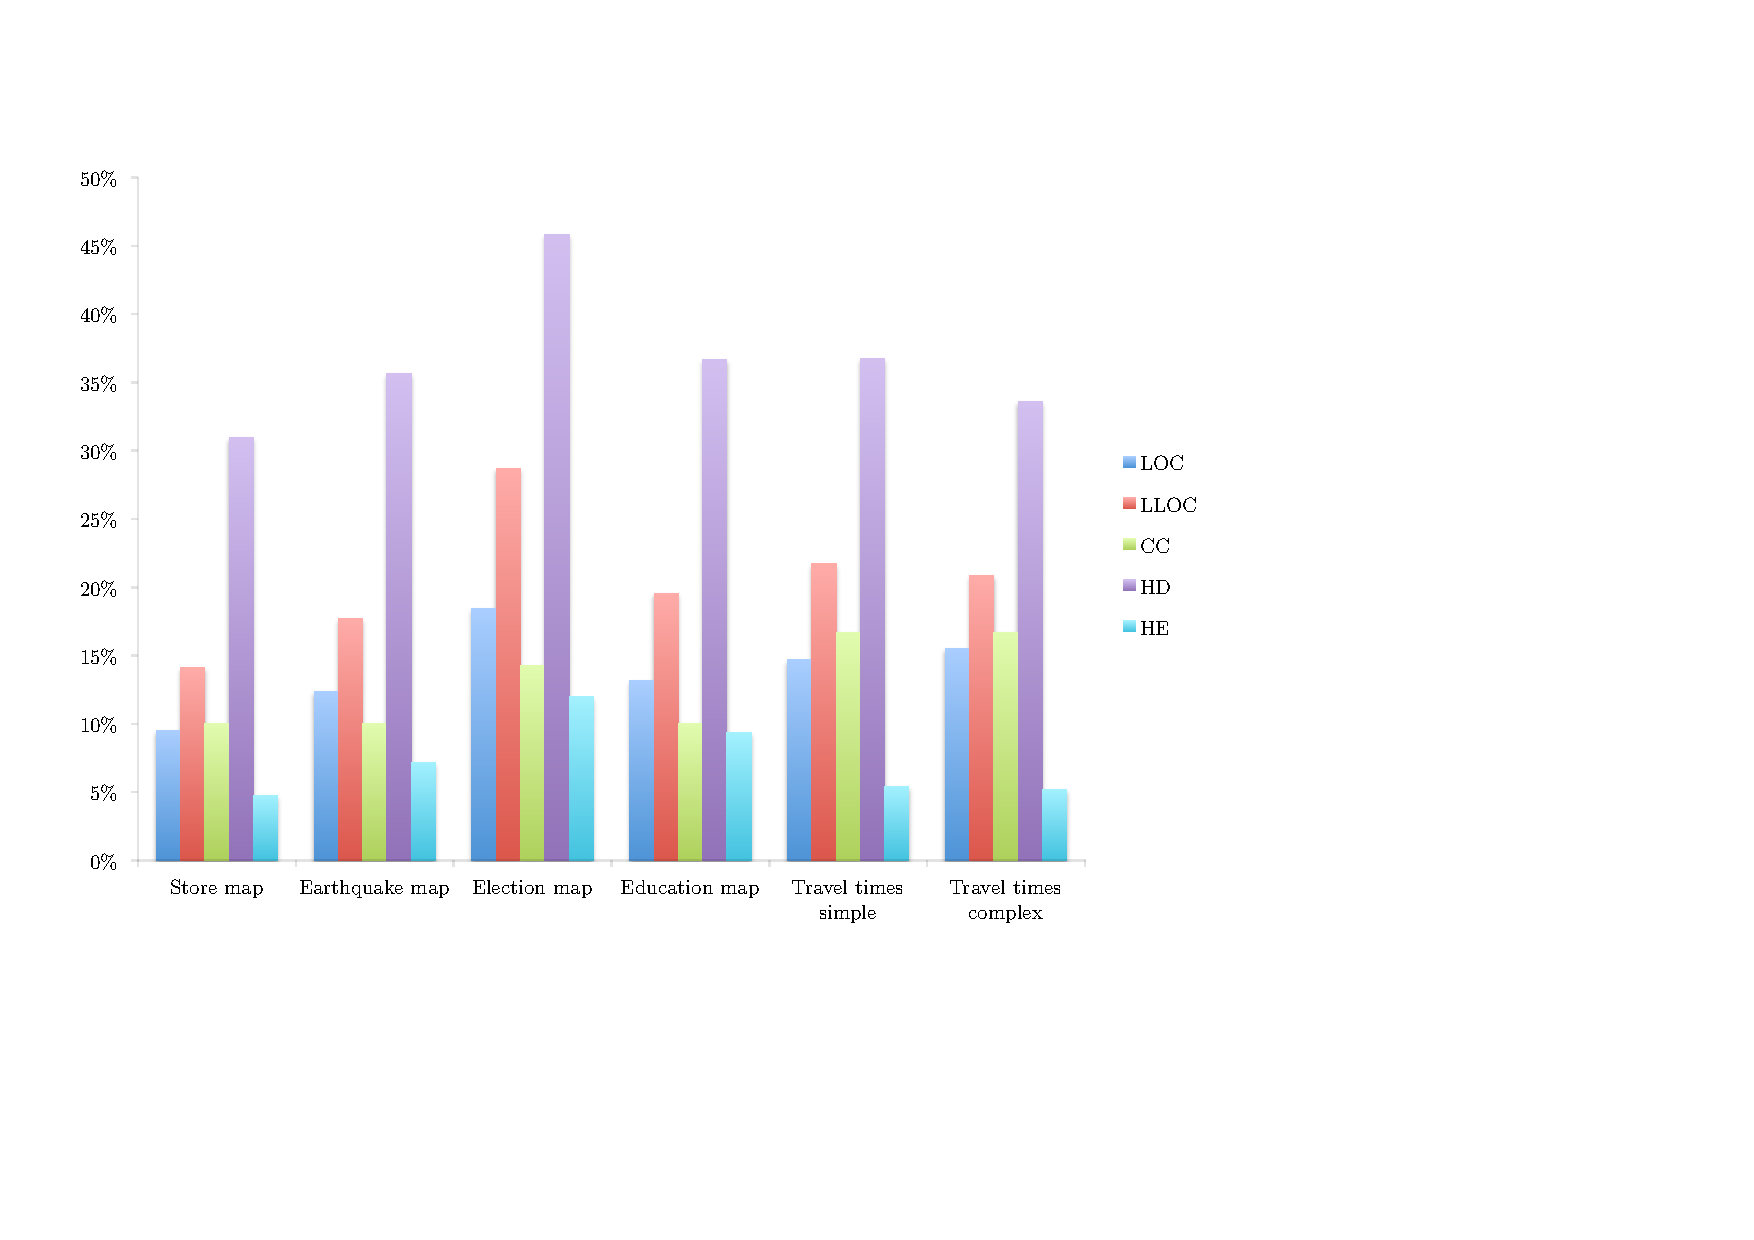
\includegraphics[width=\textwidth]{images/evaluation-results.pdf}
    \caption{Thematic.js visualization metrics for each case as a percentage of the corresponding reference visualization metric. The percentages are calculated using the values for each visualization case in table \ref{table:efficiencymetrics}}.
    \label{fig:evaluationchart}
  \end{center}
\end{figure}

Figure \ref{fig:evaluationchart} displays the ratio of Thematic.js visualization metrics for each visualization case to reference visualizations. These values are calculated using the determined values for each visualization case as presented in table \ref{table:efficiencymetrics}. The resulting metrics provide a good overview of the effort needed for Thematic.js visualizations compared to using no visualization library.

Perhaps surprisingly, according to the results, using Thematic.js yields relatively high benefits for all metrics for the dot map visualization (store map). The reason for this may be that, even though dot map is an inherently simple visualization method, e.g., error handling and marker clustering support add complexity to the reference implementation. Moreover, as the Thematic.js visualization implementation for dot map visualization consists of only 12 lines of relatively simple code, the boilerplate code needed in the reference implementation causes the relative metrics to be notably low.

Relative metrics of proportional symbol (earthquake) map are approximately similar to the metrics of dot map. However, as the proportional symbol map is missing clustering support but involves symbol scaling functionality which is also needed in the Thematic.js implementation, the relative metrics are slightly more favorable to the reference implementation than in the dot map case. Nevertheless, also in the proportional symbol case, using Thematic.js yields significant benefits compared to using no visualization framework, with Halstead effort measurement in Thematic.js implementation being under 10 \% of the corresponding measurement in the reference implementation.

Election map case yields the least benefits of all the evaluated cases, with Halstead difficulty being almost 50 \% and Halstead effort over 10 \% of the values for the reference implementation. This is likely due to the fact that the Leaflet.js mapping library provides a comprehensive GeoJSON polygon support used with choropleth visualizations. Therefore, the additional manual implementation needed for the reference case is relatively straightforward, the most effort needed being related to the coloring and showing values, the features that need to be implemented manually also in the Thematic.js implementation. That being said, even a simple choropleth map like this benefits considerably from the Thematic.js library.

In the education map case, using Thematic.js yields slightly greater benefits than in the election map. Like the election map, the education map uses choropleth mapping technique for visualization. However, the data in this case is already combined in GeoJSON format, so no manual combining is required. In both Thematic.js and reference implementations, an external coloring functionality is used, which reduces the size of the code bases. Especially the use of external coloring functionality reduces the Thematic.js relative complexity considerably, which leads to the more significant gains when using the library than in the election map case.

Both travel time maps yield highly similar results in measurements. This is likely due to the fact that both maps use isarithmic mapping method with relatively similar data, the only difference being the need for combining several data sources in the complex case. The data combining likely results in slightly lower values in Halstead difficulty and effort. However, in both of these cases, the Halstead effort metric is notably low, indicating that the effort for visualizing with Thematic.js taking only 5 \% of the effort of the reference implementation. This is probably due to the fact that even approximated isarithmic visualization requires a complex graphics implementation not supported directly by any mapping library.

Across all cases, the Thematic.js measurements indicate more significant differences in physical lines of code than logical lines of code. This is likely due to the fact that Thematic.js API is designed to encourage functional-style, chainable operations while traditional JavaScript APIs typically are imperative and non-chainable. This is demonstrated in listing \ref{listing:chainableapi}. The chainable version can be used without line breaks, resulting in only 1 physical line of code, while with the API format in second example, it is not customary to combine the lines using only source code line. However, in practice, this has little effect on the actual effort needed as the underlying functionality stays largely similar.

\begin{lstlisting}[caption=Thematic.js API format. The code has been simplified to increase readability.,language=JavaScript,label=listing:chainableapi]
// chainable API supported by Thematic.js
map.addModule('voting', new Choropleth('percentage')
        .setScale(scale)
        .setData(data));

// non-chainable API typical for traditional
// JavaScript libraries
var module = new Choropleth('percentage');
module.setScale(scale);
module.setData(data);
map.addModule('voting', module);
\end{lstlisting}

Additionally, in all the cases, Halstead difficulty measurements in Thematic.js implementations are 30 to 50 \% of the reference implementations while corresponding Halstead effort measurements are 4 to 12 \% of the reference implementations. \emph{This reflects the fact that the reference implementations consist largely of straightforward but laborious boilerplate code such as initializing the map. Thematic.js implementations consist mostly of data-specific initialization of the visualization, which is typically less straightforward but considerably more concise.}

The results are statistically significant assuming the individual measurements are distributed normally. Using the dependent samples t-test, we determined that the difference in every evaluated metric is significant using the significance level of 1 \%.

Lastly, it should be noted that while the measurements are suitable for comparing different cases, as absolute metrics they are approximate at best. In practice, this means that it is not sensible to assume that using Thematic.js reduces the effort needed to 10 \% of the original. \emph{However, in light of these results, it seems extremely likely that using the library for visualizations similar to the evaluated cases yields considerable benefits over building the visualizations from the ground up.} For more details about the measurements, see appendix \ref{appendix:escomplex}.

\section{Evaluating Effectiveness of Visualizations}
\label{section:evaluatingeffectiveness}

In order to allow as reliable effort comparison as possible, we decided to implement the same functionality to reference visualizations as in Thematic.js visualizations. In practice, this results in the reference visualization being as similar feature-wise and visually to the Thematic.js visualization as possible. Therefore, it is not reasonable to compare the effectiveness of the corresponding reference and Thematic.js visualizations. Instead, we decided to evaluate the Thematic.js visualizations qualitatively, concentrating on how the library encourages the visualizer to create effective visualizations.

\emph{The results of the evaluation suggest that using Thematic.js may benefit the effectiveness of the visualization especially when used by inexperienced visualizers.} According to the evaluation, Thematic.js yields positive results related to 12 of the 25 visualization heuristics and 4 of the 10 objectives. The application yields negative results with only 1 of the 25 heuristics and none of the 10 objectives.

\subsection{Visualization Heuristics}

\citet{zuk_heuristics_2006} provide a list of 25 heuristics for data visualizations. These heuristics are described in more detail in section \ref{section:visualizationprinciples}. We decided to use the heuristics as a basis for evaluating the created visualizations and Thematic.js functionality. We evaluated Thematic.js using a three-step scale: positive if the system has a positive effect (encourages conforming to the heuristic) when compared to using no visualization library, neutral if the system has no effect, and negative if the system encourages creating ineffective visualizations. This was done to reduce the effects of the inherently subjective research method; with only three steps, the results are explicitly approximate but less likely to suffer from subjective evaluation. The evaluation results are outlined here. The full results, along with the reasoning, can be seen in appendix \ref{appendix:heuristicsevaluation}.

Almost all heuristics yield a nonnegative result. According to the results, Thematic.js yields a positive result (encourages the visualizer to conform to the heuristic) in 12 of the 25 criteria, such as preserving action history and displaying details of the data on demand using popups. Using Thematic.js yields a neutral result (has no effect on conforming to the heuristic) in another 12 cases. Only one case was deemed negative: in some cases, Thematic.js encourages the visualizer to unnecessarily increase graphical dimensionality by visualizing scalar data in a non-scalar fashion, such as when using the proportional symbol method. The overview of the heuristics evaluation can be seen in table \ref{table:heuristicsevaluationoverview}.

\begin{table}[htb]
\centering
\begin{tabular}{|c|c|c|}
\hline
\textbf{Positive} & \textbf{Neutral} & \textbf{Negative} \\ 
\hline
Size variation & Visual variable & Graphic dimensionality \\
Most data & Color order & \\
No extra ink & Color size & \\
Gestalt laws & Local contrast & \\
Levels of detail & Color blindness & \\
Integrate text & Preattentive benefits & \\
Overview first & Zoom and filter & \\
Details on demand & Relate & \\
Extract & Uncertainty & \\
History & Relationships & \\
Multivariate & Domain Parameters & \\
Hypotheses & Cause \& effect & \\
\hline
\end{tabular}
\caption{The overview of evaluation based on the 25 heuristics presented by \citet{zuk_heuristics_2006}.}
\label{table:heuristicsevaluationoverview}
\end{table}

\emph{The heuristics evaluation indicates that using Thematic.js may be beneficial to the effectiveness of the visualization. However, this is likely dependent on the visualizer.} An experienced visualizer will probably build visualizations which conform to the heuristics as well or even better without the library. However, for inexperienced visualizers, using the library is likely beneficial for building effective visualizations. 

\subsection{Thematic Mapping Objectives}

\citet{schlichtmann_visualization_2002} provide a list of objectives for thematic mapping. These objectives are covered in more detail in section \ref{section:thematicmaps}. We evaluated the Thematic.js library by examining whether the library encourages the visualizer to achieve the objectives or not. Like in the previous section with heuristics, we employed a three-step scale for evaluation. Result for each objective is regarded as \emph{positive} if the library encourages achieving the objectives better than a typical non-visualization mapping library does. Result is regarded as \emph{neutral} if using Thematic.js has no effect on achieving the objective, and \emph{negative} if Thematic.js discourages the visualizer to achieve the objective. The results are presented in full detail in appendix \ref{appendix:objectivesevaluation}, with overview below.

Table \ref{table:objectivesevaluationoverview} displays the number of positive, neutral and negative results related to the objectives. Most of the results are regarded as neutral. This is likely due to the fact that many mapping libraries, such as Leaflet.js, already provide satisfactory level of support for many of the objectives. Therefore, using Thematic.js provides no additional benefit related to these objectives. Nevertheless, Thematic.js achieves a positive result for 4 out of 10 objectives. These are mostly due to providing explicit support for features encouraging effective visualizations, such as defining different symbols for different topeme types. It is also notable that none of the results are regarded as negative.

\begin{table}[htb]
\centering
\begin{tabular}{|c|c|c|c|}
\hline
\textbf{Positive} & \textbf{Neutral} & \textbf{Negative} \\ 
\hline
Clarification & Emphasis & \\
Types of entries & Sets of Types & \\
Cross-relations & Local syntax & \\
Addable and non- & Local ensembles & \\
addable quantities & Multilocal ensembles & \\
& The surface illusion & \\
\hline
\end{tabular}
\caption{The overview of evaluation based on objectives presented by \citet{schlichtmann_visualization_2002}.}
\label{table:objectivesevaluationoverview}
\end{table}

\emph{Thematic mapping objective evaluation hints that using Thematic.js may be beneficial to the effectiveness of resulting visualizations}. However, as with the heuristics results, this does not imply that Thematic.js is beneficial for every visualizer. An experienced visualizer may not benefit from the library in terms of effectiveness. However, especially for less experienced visualizers who might not recognize the objectives by heart, Thematic.js is probably beneficial.

 
%!TEX root = thesis.tex

\chapter{Discussion}
\label{chapter:discussion}

In this chapter, we discuss the applicability and validity of the results along with potential shortcomings of this thesis. By internal validity, we mean the validity and appropriateness of the used methods for evaluating the use cases. By external validity, we mean the generalizability of the results, i.e., whether the evaluation results can be generalized for other use cases. We also define a number of relevant aspects not covered by this research to be further studied in the future.

\section{Interpretation of Results}

\emph{Thematic.js proves that it is possible to create a reusable tool for geographical visualization.} Moreover, the results of the evaluation indicate that such tool can benefit a) the effectiveness, and b) the efficiency of visualizations. Therefore, using a tool such as Thematic.js is most likely beneficial in typical visualization cases, such as the ones demonstrated in chapter \ref{chapter:evaluation}.

As \citet{boehm_managing_1999} and \citet{mohagheghi_quality_2007}, among others, conclude, software reuse is likely to benefit the resulting software in terms of effort. This is in line with our findings. Moreover, the study by \citet{bostock_protovis:_2009} suggests that when applied appropriately, reuse may have a positive effect on the effectiveness of the visualizations. Our evaluation indicates that this is also applicable to geographical visualizations. By considering the visualization effectiveness when building the geovisualization tool, it is possible to enable visualizers using the tool to build more effective visualizations by encouraging the visualizers to adhere to heuristics for effective visualization and to achieve the objectives of thematic mapping.

%\begin{itemize}
%	\item What has been found? (A library for building visualizations can be created?)
%	\item Interpretation of the findings: it makes sense to use the reusable thingy in certain situations
%	\item Are the findings in line with the literature? (Yes, the literature also hints that the findings are appropriate) How about literature about effective visualizations? Does using a library benefit the effectiveness? Maybe use some GIS studies related to the effectiveness?
% \end{itemize}

\section{Applicability of Results}

\emph{Thematic.js provides two primary benefits for the visualizer. First, it makes building the visualization more efficient.} This quality is emphasized for less-experienced web developers as discussed in chapter \ref{section:evaluatingefficiency}. \emph{Second, it enables building more effective visualizations.} These characteristics make using the library beneficial especially for less-experienced visualizers as discussed in chapter \ref{section:evaluatingeffectiveness}.

At its current state, Thematic.js provides only a predefined set of visualization methods and thus it is not suitable for all visualization cases. Therefore, Thematic.js is most effectively used in systems requiring some of the visualization methods provided out-of-the-box. In those cases, it is highly effective in reducing the effort needed and providing high quality visualization methods. Typically, reduction in the effort needed also reduces software development costs, making Thematic.js beneficial for business purposes. 

According to a study by \citet{nambisan_technical_1999}, a major adoption barrier for web technology is the lack of knowledge about the requirements for development. Moreover, \citet{butler_barriers_2002} describe time to learn new technology and difficulty in using the technology as major obstacles for adopting new technology. Therefore, it is possible that enabling easy creation of quality visualizations may increase the number of visualizations built for all purposes. In the bigger picture, this likely benefits the general understanding of complex geographical phenomena.

Furthermore, the evaluation results related to benefits for effectiveness of Thematic.js suggest that visualization reuse may be highly beneficial also in the general level. It may be possible for the developer of reusable visualization tool to enforce ``good'' visualization practices like it is possible for the developer for reusable software to enforce good software practices such as architecture \citep{mohagheghi_quality_2007}.

% Sami: ``Eli mihin niitä vois soveltaa... esim. minkälaisiin projekteihin?, business näkökulma (koodauksesta nopeampaa?), laaja soveltaminen voi lisätä karttasovellusten tarjontaa?''

\section{Internal Validity of the Study}
\label{section:internalvalidity}

According to most of the literature presented in chapter \ref{chapter:reuse}, measuring software reuse is extraordinarily difficult. We identified several aspects potentially hindering the reusability evaluation and its validity.

The evaluation metrics used assume that the visualizer is equally acquainted with all the libraries and APIs used. However, in practice, this is unlikely. We assume that a typical visualizer creating web geovisualizations possesses at least an elementary knowledge of JavaScript APIs. Some visualizers may also have experience on using Leaflet or other mapping libraries. On the other hand, it can safely be assumed that most developers do not possess knowledge of Thematic.js beforehand. 

Therefore, it is likely that for typical visualizer, difference in effort between using and not using Thematic.js is smaller than what is indicated in the evaluation results. In order to address this issue, a study of typical web visualizers' experience would be needed. However, due to the scope of this work, we were unable to conduct this study.

Furthermore, as literature (e.g., \citealt{frakes_success_1994,mohagheghi_quality_2007}) indicates, it is unclear how the reusable parts of software should be taken into consideration when measuring characteristics of a software system. While some sources (including, e.g., \citealt{frakes_software_1996,selby_enabling_2005}) advocate including (parts of) reused software in the calculations, we decided to exclude third-party libraries. This was primarily done because we assumed that Thematic.js or other libraries were not to be modified internally, and therefore, to an external developer, they appear similar to, e.g., the standard JavaScript API. In order for this assumption to be reasonable, the documentation and functionality of the library must be thorough and reliable. Secondarily, the costs incurred while developing the library are considered as sunken and therefore do not affect the calculations.

We also decided to exclude any HTML or CSS code from the calculations. This was done primarily due to two reasons. First, in the example cases, the HTML and CSS included was almost identical due to similar requirements and the fact that Thematic.js does not provide almost any HTML-level functionality. Second, in reality, the requirements for HTML and CSS may vary considerably due to, e.g., integrating the visualizations to an existing web application. Additionally, no widely established method for measuring effort needed for building single-page web applications exists: while, e.g., \citet{mendes_web_2001} propose a metric for estimating total web development effort, the metric is mainly suitable for traditional multi-page web documents instead of single-page web applications.

For evaluation, we implemented several different geovisualizations. However, all evaluation cases were implemented by a developer who knows the library functionality along with evaluation methods and metrics. This introduces a potential selection bias which may have an influence on the results as \citet{kitchenham_evaluating_1998} correctly observe. A better alternative for this would be repeating the evaluation with several external developers. However, different developers likely have different abilities and experience on JavaScript, mapping and geovisualizations. Therefore, as \citet{mohagheghi_quality_2007} argue, for this kind of study to be reliable, the sample size should be increased considerably. This was deemed infeasible in the scope of this thesis.

As \citet{schlichtmann_visualization_2002} and \citet{slocum_thematic_2014} state, designing and building a visualization involves considerably more than just the technical construction of the map. \citeauthor{schlichtmann_visualization_2002} provides a six-step process of which only steps 4 and 5 involve the actual building of the visualization. Similarly, of the five-step process of \citeauthor{slocum_thematic_2014}, only step 5 involves building the visualization. The remaining steps were not considered in any way in the evaluation part of this work. While it can be argued that the technical means used do not affect the remaining steps, the claim could be validated for extra credibility.

%\begin{itemize}
	%\item Evaluation assumes that all APIs are equally known for the visualizer DONE
	%\begin{itemize}
	%	\item This likely not true
	%	\item The difference between known and unknown APIs -- if JS (and Leaflet) is known, but Thematic.js is not? How does this affect the true effort?
	%	\item Would need research on the average visualizer -- does she know JS or Leaflet?
	%\end{itemize}
	% \item Different evaluation methods yield different results (should the framework be included in calculations? how?) What measurements are used? Etc.
	%\begin{itemize}
	%	\item Building the library incurred costs
	%	\item The library itself likely needs maintenance etc.
	%	\item From the visualizer perspective, these do not affect much
	%\end{itemize}
	%\item Framework is reusable - how is that taken into account when calculating results (can be used in the future infinity times)
	%\item At the moment not comparing HTML, CSS etc.
	%\item Now all the implementations were done by the same guy -- the one who nows the library API and its capabilities
	%\begin{itemize}
	%	\item Better option would be to try this with external developers -- some with the tool and some without
	%	\item However, external developers likely have varying experience on JS, mapping etc.
	%	\item In order for this kind of study (with ext devs) to be reliable, sample size should be several (dozen) people (reference for this page 34 of this thesis?). This was not feasible in the scope of the thesis.
	%\end{itemize}
	%\item How about using this long term? If the visualizer gets to know the library, he will be more productive with it.
%\end{itemize}

\section{External Validity of the Study}

In addition to potential issues with the methods used, we have identified a number of potential issues regarding the generalizability of the results. These issues are discussed below.

Thematic.js along with its visualization methods were built using geovisualization literature to determine the visualization methods and functionality. We also used partly the same literature to evaluate the library. Therefore, the results are likely slightly biased towards preferring Thematic.js. While this is unfortunate, it is an essential side-effect for using the most comprehensive literature for both implementing and assessing the functionality. Moreover, for the evaluation, we complemented the criteria with additional literature sources, namely heuristics of \citet{zuk_heuristics_2006}, to minimize the bias.

Second, the selection of visualization cases for evaluation likely has an effect on the results. For the evaluation of Thematic.js, we selected a rather small number of cases using different mapping methods in order to keep the scope manageable. However, as \citet{frakes_success_1994} point out, benefits of software reuse typically increase with larger sample sets. Therefore, using, e.g., a large number of relatively similar visualization cases, the perceived benefits of the library would likely increase considerably. On the other hand, using a number of cases with more rarely used mapping methods not supported directly by Thematic.js, the perceived benefits would diminish. We did not discover means to overcome this issue. Instead, we decided to keep the number of cases rather small, while ensuring large variety among cases, and address the concern here.

Third, the visualization cases represented in evaluation are inherently simple. None of the cases employ multiple different mapping methods. Furthermore, none of the cases require complex interaction. These have also an effect on the evaluation results. With more complex visualization and interaction methods, the perceived relative benefits of the library will likely diminish as visualization implementations need additional functionality to cover the complexity and interaction. This concern could be addressed by developing more advanced mapping module functionality to the library.

%\begin{itemize}
%	\item The library was built using the same literature as the evaluated cases defined -- this likely makes it so that the library suits particularly well the cases.
%	\item The nature of cases picked for evaluation affects the results considerably - e.g. choosing really similar cases yields more positive results, really different cases yield more negative results - a note from one of the reuse sources that mention reuse evaluation being really hard
%	\item These are inherently simple visualizations - with more complex data or need, benefits are likely to diminish.
%\end{itemize}

\section{Further Research}

According to software reuse literature (e.g., \citealt{mohagheghi_quality_2007,frakes_success_1994}), reuse typically benefits other software (process) properties than effort, such as quality or maintainability. The evaluation of the cases in this work also suggested that this could apply in this case. However, we did not conduct an extensive study or analysis related to these qualities. However, as, e.g., \citet{kitchenham_software_1996} point out, software quality and maintainability are essential characteristics of a successful software system. Therefore, it would be highly beneficial to study the effect of reuse on these properties in the future.

Thematic.js library does not provide means for implementing interaction other than navigating the map. However, \citet{andrienko_interactive_1999}, and \citet[chap.~21]{slocum_thematic_2014}, among others, argue that visualization interaction greatly benefits especially exploratory data analysis. Due to the scope of this work, we decided not to consider interactions when defining or implementing Thematic.js. Therefore, it would be valuable to extend the tool in terms of interactivity in the future.

As concluded in chapter \ref{chapter:evaluation}, the profile of visualizer affects the suitability of Thematic.js for visualization. When evaluating the tool, we made assumptions about the potential users of the tool: we assumed that visualizers possess an elementary level of web development experience, along with at least some cartography experience. However, we did not base these assumptions on any specific study. While, e.g., \citet{slocum_thematic_2014} argue that the typical geovisualizer is no longer necessarily a cartographer, they do not provide any specific data about visualizers. Therefore, it would benefit the development of reusable visualization tools to conduct a study on the demographics of geographic visualizers. 

%\begin{itemize}
	% \item Framework likely affects other properties of visualizations - quality, maintainability etc. These could be studied in the future.
	% \item Interaction not covered. Software does not provide any complex interaction etc. These still need some manual coding.
	% \item Analysis on average visualizers -- are they cartographers, web developers, laymen? These qualities likely affect the library requirements (and most suitable metrics) -- another option would be creating a separate libraries (interfaces) for all three groups
	% \item How about using this long term? If the visualizer gets to know the library, he will be more productive with it.
%\end{itemize}
 
%!TEX root = thesis.tex

\chapter{Conclusions}
\label{chapter:conclusions}

In this thesis, we studied the effects of a reusable web geovisualization tool on the effort needed for building visualizations, and on the quality of the resulting visualizations. In order to do this, we studied software reuse and geovisualizations, implemented a reusable web geovisualization tool and evaluated the tool against visualizations built without it. \emph{Our principal findings were that the tool enables visualizers to build more effective visualizations more efficiently at least in certain situations}. According to our findings, the tool is beneficial especially for inexperienced visualizers and visualizers with data which is naturally visualized using the most frequently used mapping methods.

Geographical data is data with a geospatial dimension, such as Point of Interest with location data as coordinates. When such data is visualized based on the geospatial dimension, the resulting visualization is called \emph{geographical visualization} (or \emph{geovisualization}). Most typically, geographical visualization is done using a map using the process called \emph{thematic mapping}. In the past, thematic maps were predominantly made by cartographers. However, recently, the advent of web-based mapping tools has enabled non-cartographers to create various map visualizations. Currently, it is estimated that the majority of web map visualizations are made by laymen with no education related to cartography.

% While the definition of visualization is disputed, visualizations can be measured in several ways. According to \citet{tufte_visual_1986}, visualizations should, above all, show the data consistently. This is a valuable guideline, but too vague for exact measurements. For more concrete guidelines, \citet{zuk_heuristics_2006} present a number of heuristics for evaluating visualizations. The heuristics consist mainly of psychological guidelines applied for visualization use.

% Thematic maps can be created using a number of \emph{mapping methods}. Choropleth map is the most frequently used mapping method. Choropleth maps consist of predefined enumeration areas (e.g., countries or municipalities) for which a uniform visualizable property (e.g., median income) can be determined. Isarithmic maps are visualizations depicting smooth or continuous phenomena, such as elevation. In isarithmic map, phenomena are typically visualized using gradients, often accompanied by \emph{contour lines}. Dot maps and proportional symbol maps are used to display phenomena related to point location, typically with dots or markers placed to the locations. Additional widely used mapping methods include dasymetric maps, cartograms and flow maps. Additionally, a single geographic visualization can consist of several different mapping methods.

% Software reuse has great potential. When applied appropriately, it typically results in a considerably reduced need for effort and higher quality. However, the benefits of reuse are difficult to measure. Typically, software reuse benefits primarily on long-term; on short-term, it may be perceived as disadvantageous. Several methods exist for creating reusable software. Scavenging is an \emph{ad hoc} reuse method in which code and other assets are copied from code base to another as is. Source code components are built as reusable pieces of software with explicit interfaces for integration. Application generators are programs designed to output another program according to high-level specifications. Software frameworks combine software components and programming patterns to provide a comprehensive approach for reuse. Typically, several of the methods can be used together.

Before this work, apart from general-purpose mapping libraries, practically no libraries exist for building geovisualizations on the web. General-purpose mapping libraries such as Google Maps API support building visualizations to some degree. However, these libraries are of too low abstraction level to allow building more complex visualizations efficiently. Moreover, as the libraries are not designed for building visualizations, they do not encourage building effective visualizations. Therefore, it is both laborious and difficult to build effective map visualizations with general-purpose mapping tools. Moreover, research on the effect of software reuse on the quality of visualization is scant.

During this work, we implemented Thematic.js, a reusable visualization application for the web. The application can be used independently as a single-page application, or as a part of other JavaScript applications. The application is designed to support the most frequently used thematic mapping methods and relevant utility functionality. Additionally, the application architecture is designed to be modular for efficient extensibility.

We evaluated the implemented application by defining several use cases depicting typical geovisualization use. Then, we implemented the cases using Thematic.js, and reference implementations for comparison using Leaflet.js, a general-purpose mapping library. These implementations were then compared using several metrics for software development effort. Additionally, we evaluated the Thematic.js implementations according to the visualization heuristics of \citet{zuk_heuristics_2006} and mapping objectives of \citet{schlichtmann_visualization_2002}.

\emph{The evaluation results indicated that using Thematic.js, building geographic visualizations is significantly less laborious.} In the test cases evaluated, implementations built with Thematic.js required an average of 7 \% of the effort needed for the reference implementation. Moreover, Thematic.js implementations used only 14 \% of physical and 20 \% of logical lines of code, introduced 13 \% of the complexity and 37 \% difficulty when compared to reference implementations. The results are statistically significant using the Student's t-test with a significance level of 1 \%.

Additionally, we deemed using Thematic.js beneficial regarding 16 of 35 visualization effectiveness guidelines (heuristics and objectives), with only 1 of 35 guidelines deemed negative. \emph{This indicates that Thematic.js is beneficial to the effectiveness of the visualization at least in certain cases.}

Thus, we can conclude the findings in relation to the research questions selected:%\vskip 2em
% FIXME ensure that this renders correctly

\begin{enumerate}
	\item[RQ1] How does a reusable software system affect the \emph{efficiency} of building geographical visualizations?
	\item[A1] According to our findings, a reusable software system such as Thematic.js increases the efficiency of building geographical visualizations considerably.
\end{enumerate}
\begin{enumerate}
	\item[RQ2] Can a reusable software system enable creating \emph{effective} geographical visualizations?
	\item[A2] According to our findings, a reusable software system such as Thematic.js encourages visualizers to create effective geographical visualizations.
\end{enumerate}

While the results look highly promising, reliable effort measurement is incredibly hard. Therefore, we presented a number of concerns regarding the validity of results. First, the correct level of inclusion of reusable parts of a software system for measurements is disputed. We decided to exclude the reusable parts. Measurements with reusable parts included would likely yield more negative results regarding the effort needed. Second, the metrics do not take into consideration different experience levels of visualizers and thus the results may vary greatly depending on the visualizer. Third, while the use cases were selected according to approximate usage of visualization methods, using different methods would probably yield highly different results: evaluating methods which are not supported by Thematic.js is likely to yield considerably less promising results.

To conclude, we suggest that visualizers consider using Thematic.js in projects requiring web-based geographical visualizations. It is likely that Thematic.js benefits such projects regarding both development efficiency and visualization effectiveness.



% Load the bibliographic references
% ------------------------------------------------------------------
% You can use several .bib files:
% \bibliography{thesis_sources,ietf_sources}
\fixme{Hand-check references, remove google books urls, consolidate accessed dates, etc.}

\bibliography{sources,sources_example}


% Appendices go here
% ------------------------------------------------------------------
% If you do not have appendices, comment out the following lines
\appendix
%!TEX root = thesis.tex

\chapter{Flat Dot Format}
\label{appendix:flatdotformat}

Flat dot format is a simple, but non-standard format used by a number of web mapping applications such as the Store Finder of Alko\footnote{\url{http://www.alko.fi/myymalat/}}. Format consists of a JSON\footnote{\url{http://www.json.org/}} file representing an array of zero or more objects. The objects must contain latitude and longitude properties, and may contain a number of other properties. An example of the format is depicted below.

\begin{lstlisting}[language=JavaScript]
[
  {
    "number": 2,
    "name": "Destination",
    "latitude": 60.314322,
    "longitude": 24.554067
  },
  {
    "number": 0,
    "name": "Departure",
    "latitude": 60.314041,
    "longitude": 24.551678
  },
  {
    "number": 1,
    "name": "Pit stop",
    "latitude": 60.316474,
    "longitude": 24.556554
  }
]
\end{lstlisting}

\chapter{ESComplex Results for Visualizations}
\label{appendix:escomplex}

For the sake of conciseness, I omitted the full output of ESComplex\footnote{\url{https://github.com/philbooth/escomplex}} tool for evaluated cases in JSON format. The output contains additional details about the measurements, such as the full operator and operand lists. The full results are available in \url{https://github.com/pyryk/thesis-evaluation-results}.

\chapter{Visualization Heuristics Evaluation}
\label{appendix:heuristicsevaluation}

Thematic.js evaluation results based on the visualization heuristics presented by \citet{zuk_heuristics_2006} are displayed in table \ref{table:heuristicsevaluation}. The evaluation was done using a tree-step scale. Heuristic is evaluated \emph{positive} if Thematic.js encourages conforming to the heuristic when compared to using no visualization library, \emph{neutral} if using Thematic.js has no effect, and \emph{negative} if Thematic.js discourages conforming to the heuristic.

\begin{longtable}{|p{3cm}|p{2.2cm}|p{7.8cm}|}
\hline
\textbf{Heuristic} & \textbf{Evaluation} & \textbf{Reasoning} \\
\hline
\endhead
\hline
\endfoot
\endlastfoot
Visual variable & Neutral & Of map visualizations, this concerns mostly choropleth maps. Thematic.js choropleth maps do not ensure minimum geographical size for areas. However, using the default line weight ensures a minimum screen size of several pixels. \\[0.5em] % Ensure visual variable has sufficient length \\
Color order & Neutral & Thematic.js choropleth, dasymetric and isarithmic maps are primarily based on coloring the map. Moreover, the visualizer is given the possibility of freely choosing the colors. This may lead to situations when the visualizer chooses the colors inappropriately for displaying order. However, this situation is not different from the alternative situation of the visualizer creating the visualization without using a visualization library. \\[0.5em] % Don't expect a reading order from color \\
Color size & Neutral & Thematic.js does not provide any color-adjusting mechanisms based on the size of the element. \\[0.5em] % Color perception varies with size of colored item
Local contrast & Neutral & Thematic.js does not provide any color-adjusting mechanisms based on contrast. \\[0.5em] % Local contrast affects color
Color blindness & Neutral & Thematic.js does not provide any advice regarding color blindness. \\[0.5em] % Consider people with color blindness
Preattentive benefits & Neutral & Thematic.js provides and enforces spacial positioning of the data. However, this is fundamental to any geovisualization, and therefore, cannot be considered a positive trait of the library. \\[0.5em] % Preattentive benefits increase with field of view
Size variation & Positive & Thematic.js provides size variation in proportional symbol mapping to encourage the visualizer to emphasize quantitative variation in data. \\[0.5em] % Quantitative assessment requires position or size variation
Graphic dimensionality & Negative & Thematic.js does not enforce preserving dimensionality of the data, and in some cases, such as when using a proportional symbol map, it encourages the visualizer to increase dimensionality by displaying scalar values using proportional symbols. \\[0.5em] % Preserve data to graphic dimensionality
Most data & Positive & Thematic.js encourages the visualizer to maximize data shown by providing support for several different mapping methods suitable for different kind of data. \\[0.5em] % Put the most data in the least space
No extra ink & Positive & Thematic.js provides data aggregation functionality to combine the relevant data. \\[0.5em] % Remove the extraneous (ink)
Gestalt laws & Positive & Thematic.js provides functionality to support Gestalt laws of grouping, such as using different symbols and sizes for different data points. However, not all Gestalt laws are considered. \\[0.5em] % Consider Gestalt Laws
Levels of detail & Positive & Thematic.js provides clustering functionality of dots and symbols. While currently there is no support for levels of detail for other mapping methods, the library does not prevent implementing this in the future. \\[0.5em] % Provide multiple levels of detail
Integrate text & Positive & Thematic.js supports attaching popups with textual content to data points, such as markers or choropleth areas. \\[0.5em]
Overview first & Positive & Thematic.js supports overview-first approach in most of the mapping methods. Dot and proportional symbol maps support marker clustering and choropleth, isarithmic and dasymetric maps support zooming for displaying the details. \\[0.5em] % Provide overview first
Zoom and filter & Neutral & Thematic.js supports zooming of the map. However, support for filtering data on view-level is not provided. \\[0.5em]
Details on demand & Positive & Thematic.js supports attaching popups to data points for displaying additional details. \\[0.5em]
Relate & Neutral & Thematic.js does not support any method of emphasizing relationships between entries other than spacial distribution. \\[0.5em] % Consider relationships among items
Extract & Positive & While Thematic.js does not support physical saving of data subsets, it provides bookmarking and linking support which effectively provide similar benefits. \\[0.5em] % Allow extraction of data and its subsets
History & Positive & Thematic.js supports using the back and forward buttons of the browser to undo and redo actions. \\[0.5em] % Keep history of actions
Uncertainty & Neutral & Thematic.js does not encourage the visualizer to display the uncertainties in data. \\[0.5em] % Expose uncertainty
Relationships & Neutral & Thematic.js does not encourage concretizing relations between data points. \\[0.5em] % Concretize relationships
Domain Parameters & Neutral & While Thematic.js modules require explicitly stating the used parameters, there is no guarantee about the importance of selected parameters. \\[0.5em] % Determination of domain parameters
Multivariate & Positive & Thematic.js provides aggregation functionality in order enable easy experimenting about relationships between variables. Moreover, the modular structure of the library results in the possibility to easily combine several visualization methods to highlight different aspects of the data. \\[0.5em] % Provide multivariate explanation
Cause \& effect & Neutral & Thematic.js does not provide additional means for determining or displaying cause and effect. \\[0.5em] % Formulate cause & effect
Hypotheses & Positive & The availability of several different mapping methods of Thematic.js encourage the visualizer to better display and evaluate hypotheses. \\[0.5em] % Confirm Hypotheses
\hline
\caption{Evaluation of Thematic.js according to heuristics presented by \citet{zuk_heuristics_2006}.}
\label{table:heuristicsevaluation}
\end{longtable}

\chapter{Mapping Objectives Evaluation}
\label{appendix:objectivesevaluation}

Evaluation results of Thematic.js regarding thematic mapping objectives of \citet{schlichtmann_visualization_2002} are presented in table \ref{table:objectivesevaluation}. The evaluation was performed with a three-step scale. Result for each objective is regarded as \emph{positive} if the library encourages achieving the objectives better than typical mapping library does. Result is regarded as \emph{neutral} if using Thematic.js has no effect on achieving the objective, and \emph{negative} if Thematic.js discourages the visualizer to achieve the objective.

\LTcapwidth=\textwidth
\begin{longtable}{|p{3cm}|p{2.5cm}|p{7.5cm}|}
\hline
\textbf{Name} & \textbf{Evaluation} & \textbf{Reasoning} \\ 
\hline
\endhead
\hline
\endfoot
\endlastfoot
% Making the map clear and readable. In practice, this means that the topemes (symbols) in a map should be easily detectable and distinguishable from each other
Clarification & Positive & Thematic.js benefits the clarification of the visualization by, e.g., providing clustering functionality of the markers \\[0.5em]
% Making topemes and other important characteristics of the visualization to stand out visually
Emphasis & Neutral & Thematic.js uses visual markers in dot maps. However, this is typically achieved with any mapping library even with no visualization library. \\[0.5em]
% Having a clearly distinguishable type for each topeme.
Types of Entries & Positive & Thematic.js provides support for using different markers for different types of topemes. \\[0.5em]
% Grouping data points and symbols with similar traits in order to make them belong together visually. Ideally, the visual similarity should be related to the conceptual similarity.
Sets of Types & Neutral & Thematic.js does neither encourage nor discourage consolidating types of topemes according to mutual similarities. \\[0.5em]
% Visually indicating the potential relations and similarities between different types or between entries of different types.
Cross-Relations & Positive & Several of the mapping methods, especially proportional symbol method, support indicating similarities between different types of entries. \\[0.5em]
% Aligning visual properties of the topemes to prevent unintentional emphasis of single topemes.
Local Syntax & Neutral & Thematic.js pays no special attention to managing lower-order units within topemes. \\[0.5em]
% Supporting topemes with multiple properties (such as the numbers of children and adults in an area) so that the topeme visually reflect both the individual properties and the combination of all properties.
Local Ensembles & Neutral & Local ensembles are not supported in any of the current mapping methods of Thematic.js. \\[0.5em]
% Supporting topemes with multiple geographical properties (such as spatial distribution of people)
Multilocal Ensembles & Neutral &  Multilocal ensembles are not supported in any of the current mapping methods of Thematic.js. \\[0.5em]
% Differentiating addable and non-addable properties. Typically absolute quantitative properties are addable while relative and qualitative properties are non-addable. Addable properties should be visualized in a way that cognitively supports addition (e.g., with sizes of elements) while non-addable quantities should be visualized without said feature (e.g., with colors.)
Addable and Non-Addable Quantities & Positive & Thematic.js separates between addable and non-addable quantities by separating between different mapping methods. \\[0.5em]
% Creating an illusion of surface on the map. This can be achieved for example by using illumination and shadowing. These visual traits can convey a meaning themselves and often naturally do so.
The Surface Illusion & Neutral & Thematic.js provides no additional means of achieving the surface illusion when compared to, e.g., the underlying Leaflet.js mapping library. \\[0.5em]
\hline
\caption{Evaluation of Thematic.js according to the map visualization objectives of \citet{schlichtmann_visualization_2002}.}
\label{table:objectivesevaluation}
\end{longtable}

% End of document!
% ------------------------------------------------------------------
% The LastPage package automatically places a label on the last page.
% That works better than placing a label here manually, because the
% label might not go to the actual last page, if LaTeX needs to place
% floats (that is, figures, tables, and such) to the end of the 
% document.
\end{document}
